\chapter{Bots basados en árboles de decisión}

\section{Idea general}
Un Árbol de Decisión es un tipo especial de árbol utilizado en el área de Inteligencia Artificial cuyos nodos internos representan condiciones a evaluar y sus nodos hoja representan las acciones a realizar, resultados, soluciones, etc. El recorrido de un Árbol de Decisión es sencillo, se empieza por el nodo raíz y se evalúa su condición, dependiendo del resultado de esta evaluación se elige el siguiente nodo (hijo del nodo evaluado) que será evaluado y así sucesivamente hasta que se encuentre un nodo hoja.
\begin{figure}[H]
\centering
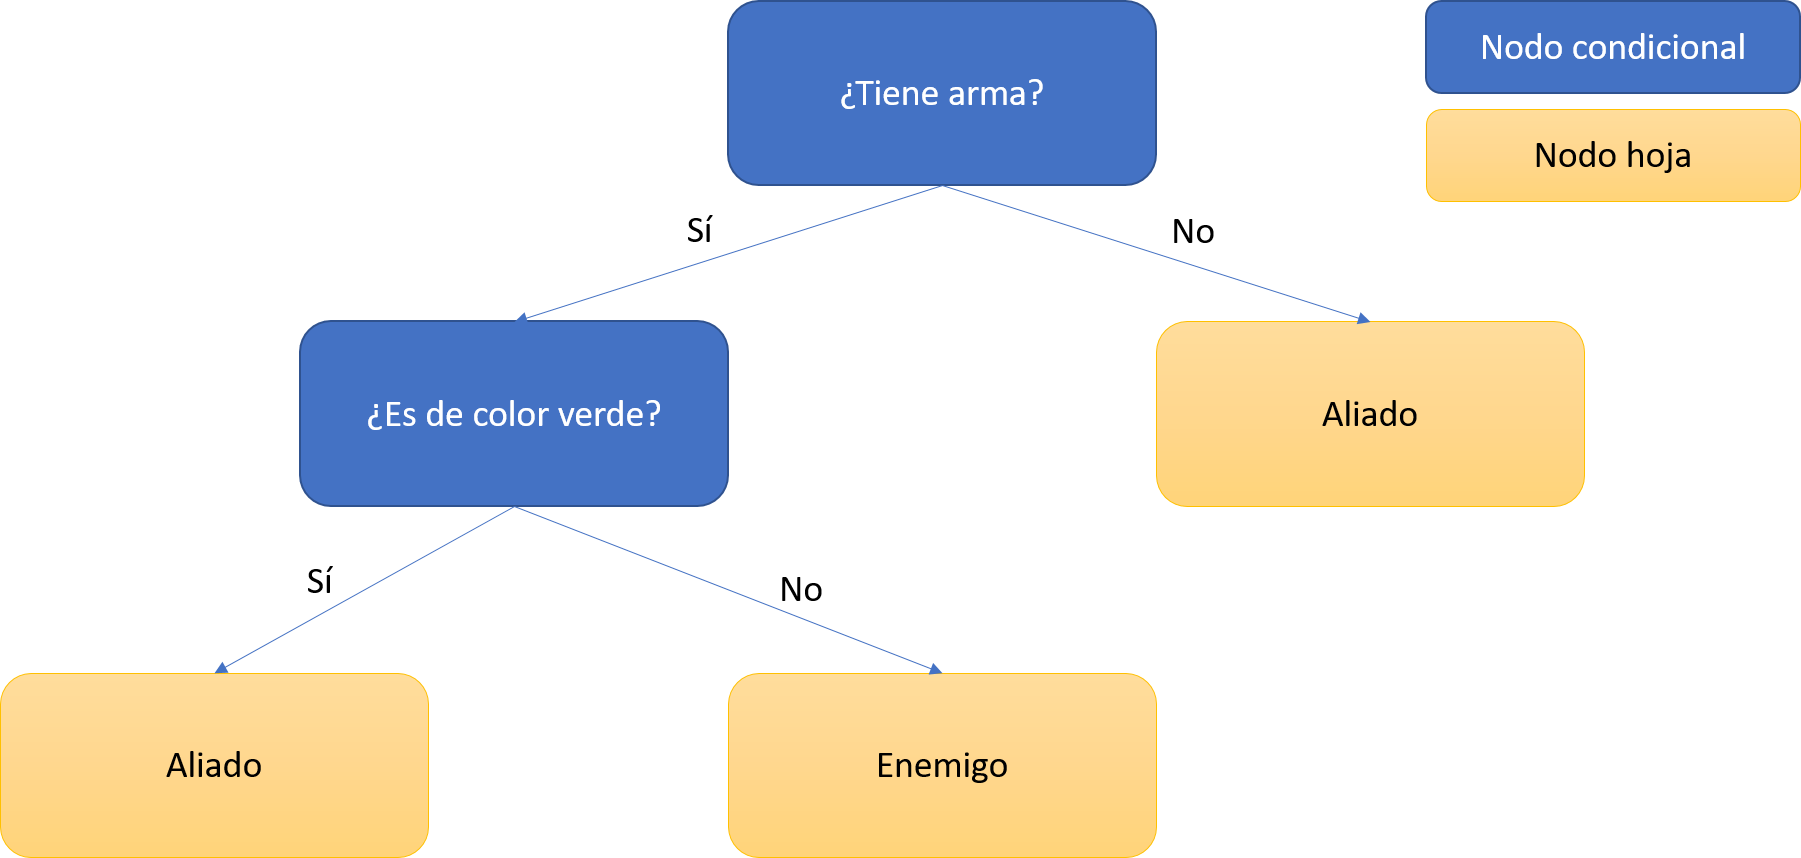
\includegraphics[width=\textwidth]{arbol-decision}
\caption{Árbol de decisión para determinar si un individuo es enemigo o aliado.}
\end{figure}

Los Árboles de Decisión suelen emplearse ampliamente en áreas donde sean necesarias decisiones deterministas automatizadas como finanzas, estadística, videojuegos, aprendizaje automático, etc. Son fáciles de entender y muy rápidos de procesar una vez construidos\cite{aihorizonDecisiontrees}.

En esta fase optamos por seguir un nuevo enfoque mediante Inteligencia Artificial Reactiva. Esto significa evaluar en cada turno un árbol de decisión (partiendo siempre desde la raíz), comprobando una serie de condiciones del estado de la partida, y a partir de ellas determinar una única acción a realizar. La decisión de seguir este enfoque persigue que nuestros bots resultantes tengan un comportamiento con continuidad dentro de una misma situación pero a la vez sean capaz de adaptarse a cambios repentinos en el estado del juego. 
 
Por ejemplo,a partir del código:
\begin{lstlisting}[frame=single, breaklines=no, basicstyle=\fontsize{10}{11}\ttfamily]
    if ( getDistanceToClosestNonEdibleGhost >= 4 ){
        getDirectionToClosestEdibleGhost
    } else {
        getDirectionAwayFromClosestNonEdibleGhost
    }
\end{lstlisting}

construiríamos el siguiente árbol:
\begin{figure}[H]
\centering
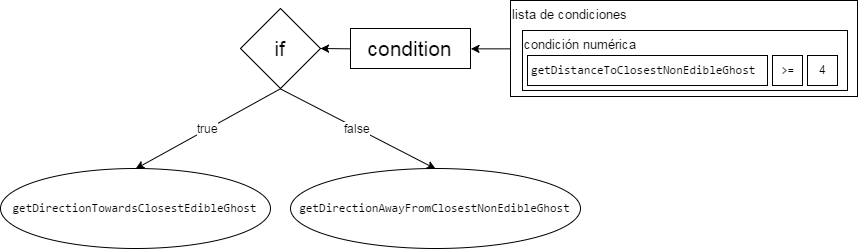
\includegraphics[width=\textwidth]{codigo-a-arbol}
\end{figure}
La ejecución de este árbol consistiría en turno a turno evaluar desde el nodo raíz: primero, comprobar si la distancia al fantasma no comible más cercano es menor o igual que 4. En caso de que sea así, evalúa la rama izquierda recursivamente, y al ser esta un nodo hoja ejecuta la acción determinada por este, en este caso acercarse al fantasma comible más cercano. En caso de la que condición no se cumpla, se ejecutará de forma análoga la rama derecha, tratándose de un nodo hoja con la acción que genera un movimiento de huida del fantasma más cercano. 

\subsection{Árboles de decisión}
Posteriormente optamos por un cambio en la representación del fenotipo. Concretamente, a partir de cada fenotipo generado por el algoritmo evolutivo, generamos un árbol de decisión para simplificar significativamente la ejecución de una partida con dicho fenotipo, y así lograr la ya mencionada Inteligencia Artificial Reactiva. Dicho árbol contiene las diferentes funciones para consultar el estado de juego (los nodos no terminales) y para decidir movimientos (nodos terminales) como enumerados, obteniéndose cada movimiento evaluando recursivamente el árbol.
 
La razón de estos árboles era poder codificar comportamientos mucho más complejos en sus diferentes ``ramas'', pudiendo además explotar la riqueza de las gramáticas, simplificar la lógica de ejecución, y desarrollar una base mucho más estable sobre la que apoyar futuras iteraciones.

\subsection{Parsing de fenotipo a árbol}
A la hora de realizar el cambio estructural de fenotipo, optamos por realizar un parsing del fenotipo desde una cadena de caracteres (producida por JECO mediante evolución gramatical) a un árbol que organiza los ya mencionados condicionales, consecuentes y movimientos de la forma más intuitiva posible. La estructuración de dichos elementos dentro del árbol se realiza de la siguiente forma:

\subsubsection{Nodos terminales}
Los nodos terminales realizan una acción o una consulta. Si es una acción puede tratarse de:
\begin{itemize}
\item Movimientos simples (direccionales)
\item Movimientos basados en información del juego. Por ejemplo, ``el movimiento que aleja más a Pac-Man del fantasma más cercano''
\end{itemize}

En el caso de las consultas al estado del juego, estas pueden devolver distancias en formato entero (distancia al fantasma comible más cercano, ...) o booleanos (¿Está Pac-Man en una intersección?, ...).

\subsubsection{Nodos condicionales}
Los nodos condicionales contienen una lista de parámetros booleanos (los cuales hemos denominado condiciones) y otra lista que indica qué operadores booleanos binarios operan dichos parámetros. En caso de tratarse de un \texttt{if}, contendrá un nodo hijo con un consecuente, y en caso de ser un \texttt{else}, dos.
 
Una condición puede ser de varios tipos, según el tipo de los parámetros que contenga:
\begin{itemize}
\item de función booleana
\item de función numérica, operador numérico (binario) y función numérica
\item de función numérica, operador numérico (binario) y número
\item de número, operador numérico (binario) y función numérica
\end{itemize}

Los parámetros de tipo función que contenga una condición una vez más se trataran de enumerados, con la diferencia de que en este caso el método que poseen indicará el valor (booleano o numérico) de la consulta del estado de alguna variable de la partida. Finalmente, una condición puede encontrarse negada.

\subsection{Adaptador de árbol a movimiento de Pac-Man}
Para poder ejecutar partidas con estos árboles de decisión, necesitamos implementar un nuevo controlador de Pac-Man. Este controlador contiene el árbol de derivación, actuando como wrapper, de forma que con cada solicitud de movimiento realizada al controlador, este evalúa el árbol de forma recursiva, hasta encontrar un nodo terminal que devuelva un movimiento y que cumple todas sus condiciones previas.

Nótese  que la evaluación de dichos condicionales supone la evaluación de numerosos parámetros booleanos y enteros evaluados entre sí. Estos parámetros son obtenidos directamente de consultas al estado de la partida.

Finalmente se obtiene un movimiento, bien generado por la acción de un nodo terminal a través de la llamada a una determinada función interna del juego Ms. Pac-Man vs Ghosts, bien realizando un movimiento simple direccional.

\section{Gramáticas desarrolladas}
Todas nuestras gramáticas producen códigos basados en inteligencias artificiales reactivas, es decir, a cada turno de movimiento (denominado internamente como \textit{tick}) se evalúan una serie de condiciones del estado del tablero para producir un único movimiento de forma no ambigua. Las gramáticas diseñadas usan una estructura de anidamientos de declaraciones \texttt{if-else} que posteriormente un \textit{parser}\footnote{Un parser es una herramienta que mediante el uso de una gramática transforma texto escrito en el lenguaje representado por la gramática a una representación interpretable por otro sistema\cite{parserTechopedia}.
} convertirá a un Árbol de Decisión. Este Árbol de Decisión tendrá una traducción directa de las funciones escritas en la Gramática a funciones interpretables por el bot (escritas en \textit{Java}) que serán ejecutadas en el proceso de evaluación.
 
A la hora de desarrollar gramáticas las dividimos en tres categorías dependiendo del tipo de acciones que pueden producir:
\begin{itemize}
\item Bajo nivel: Son gramáticas cuyos nodos terminales, aquellos que dicen al bot de Pac-Man qué movimiento hacer en cada \textit{tick} del juego, se constituyen únicamente de las funciones \texttt{Up, Down, Left, Right} que son una codificación directa de las teclas de movimiento que dispondría un humano al jugar el juego.

\item Medio nivel: Aparte de las funciones básicas de movimiento (\texttt{Up, Down, ...}), disponen de funciones de un nivel medio,  entendiéndose nivel medio como funciones que dictan una acción directa, como puede ser comerse la \textit{pill} más cercana, huir del fantasma más cercano, ir a por la \textit{power pill} más cercana, etc.

\item Alto nivel: Se diferencian de las de medio nivel en que sus funciones terminales son muy abstractas y no se puede determinar directamente qué dirección o comportamiento tomará el bot, estas funciones son del estilo de \textit{comer, huir, atacar, ...} funciones que se entienden cuál es su objetivo pero que pueden realizarse de distintas maneras.
\end{itemize}

\subsection{Parámetros del experimento realizado} \label{sec:params}
Todos los resultados de esta sección han sido obtenidos empleando los mismos operadores, parámetros y probabilidad con la que se emplean los operadores del algoritmo evolutivo para permitir una comparación objetiva del rendimiento empleando diferentes gramáticas. Estos parámetros son:
\begin{table}[H]
\centering
\begin{tabular}{lll}
\cline{3-3}
                                                         &                & \textbf{Porcentaje} \\ \cline{3-3} 
\multicolumn{1}{|l|}{\textbf{Población}}                          & 100            & -          \\
\multicolumn{1}{|l|}{\textbf{Generaciones}}                       & 100            & -          \\
\multicolumn{1}{|l|}{\textbf{Evaluaciones por individuo}} & 30             & -          \\
\multicolumn{1}{|l|}{\textbf{Longitud cromosoma}}                 & 100            & -          \\
\multicolumn{1}{|l|}{\textbf{Límite superior codón\footnotemark[2]}}              & 256            & -          \\
\multicolumn{1}{|l|}{\textbf{Método de selección}}                & Torneo Binario\footnotemark[3]& -          \\
\multicolumn{1}{|l|}{\textbf{Método de cruce}}                    & LHS            & 60         \\
\multicolumn{1}{|l|}{\textbf{Método de mutación}}                 & Integer Flip   & 10         \\
\multicolumn{1}{|l|}{\textbf{Mutación Neutral}}                   & Sí             & -          \\
\multicolumn{1}{|l|}{\textbf{Elitismo}}                           & Sí             & 5         
\end{tabular}
\end{table}
\footnotetext[2]{valor máximo que puede tomar}
\footnotetext[3]{o NSGA II si se está empleando multiobjetivo}

\subsection{Gramática de bajo nivel}
Con la gramática de bajo nivel pretendemos que el bot tenga un comportamiento basado en estímulos muy específicos y utilizando solo los operadores de movimiento de los que un jugador humano dispone (\texttt{moveup, moveDown, moveRight, moveLeft}). Como son operadores de bajo nivel que no disponen de información del juego (\textit{pill} más cercana, posición de fantasmas, etc), la gramática necesita contener una gran cantidad de funciones que devuelvan información del estado actual del juego:
\begin{itemize}
\item \texttt{getDistanceToClosestNonEdibleGhost}: Devuelve la distancia al fantasma peligroso más cercano.

\item \texttt{getDistanceToClosestNonEdibleGhost{Up, Down, Left, Right}}: Distancia al fantasma peligroso más cercano a la posición del bot en la dirección dada.

\item \texttt{getDistanceToClosestEdibleGhost}: Devuelve la distancia al fantasma comestible más cercano.

\item \texttt{getDistanceToClosestEdibleGhost{Up, Down, Left, Right}}: Distancia al fantasma comestible más cercano a la posición del bot en la dirección dada.

\item \texttt{getNumberOfActivePowerPills}: Devuelve la cantidad de \textit{power pills} que se encuentran actualmente en el tablero.

\item \texttt{getDistanceToClosestPill}: Distancia a la \textit{pill} (también considerando las \textit{power pills}) más cercana independientemente de la orientación del bot.

\item \texttt{getDistanceToClosestPill{Up, Down, Left Right}}: Devuelve la \textit{pill} más cercana al bot en la dirección especificada.

\item \texttt{getClosesPowerPill{Up, Down, Left Right}}: Idéntica a las anteriores pero teniendo en cuenta solo las \textit{power pills}.

\item \texttt{getClosestJunctionExitsNumber{Up, Down, Left, Right}} = Número de salidas de la intersección más cercana a la posición del bot en la dirección dada.

\item \texttt{getDistanceToClosestJunction{Up, Down, Left, Right}} = Distancia del bot a la intersección más cercana dada una dirección.

\item \texttt{getClosestNonEdibleGhostDistanceToClosestJunction{Up, Down, Left Right}}: Devuelve la distancia del fantasma peligroso más cercano a la intersección más cercana al bot en la dirección dada.

\item \texttt{getClosestEdibleGhostDistanceToClosestJunction{Up, Down, Left Right}}: Identica a las anteriores funciones pero con fantasmas comestibles.

\item \texttt{getGeometricMeanDistanceToNonEdibleGhosts}: Devuelve la distancia media geométrica a los fantasmas peligrosos.

\item \texttt{getGeometricMeanDistanceToEdibleGhosts}: Idéntica a la anterior pero la distancia a los fantasmas comestibles.
\end{itemize}

Los resultados de estos operadores de obtención del estado del juego se comparan dentro de las condiciones de las declaraciones \texttt{if} contra un número. Este número en vez de permitir generarlo de forma arbitraria por la gramática lo que hemos decidido es introducir nosotros un conjunto discreto de números que pueden ser escogidos para las comparaciones, reduciendo de este modo el espacio de búsqueda y la generaciones de números absurdos (extremadamente grandes).

\subsubsection{Notación BNF}
\begin{lstlisting}[frame=single, breaklines=no, basicstyle=\fontsize{10}{11}\ttfamily, caption=Gramática de bajo nivel]
<grammar> ::= <selection-statement>
 
<selection-statement> ::= if( <condition> ){ <statement> } else{ <statement> }
                        | if( <condition> ){ <statement> }
 
<statement> ::= <terminal-func>
              | <selection-statement>
 
<terminal-func> ::= <simpleMoves>
 
<condition> ::= <number-func> <number-operator> <number>
 
<number-func> ::= getDistanceToClosestNonEdibleGhost
                | getDistanceToClosestNonEdibleGhostUp
                | getDistanceToClosestNonEdibleGhostDown
                | getDistanceToClosestNonEdibleGhostLeft
                | getDistanceToClosestNonEdibleGhostRight
                | getDistanceToClosestEdibleGhost
                | getDistanceToClosestEdibleGhostUp
                | getDistanceToClosestEdibleGhostDown
                | getDistanceToClosestEdibleGhostLeft
                | getDistanceToClosestEdibleGhostRight
                | getNumberOfActivePowerPills
                | getDistToClosestPillUp
                | getDistToClosestPillDown
                | getDistToClosestPillLeft
                | getDistToClosestPillRight
                | getDistToClosestPill
                | getDistToClosestPowerPill
                | getDistToClosestPowerPillUp
                | getDistToClosestPowerPillDown
                | getDistToClosestPowerPillLeft
                | getDistToClosestPowerPillRight
                | getClosestJunctionExitsNumberUp
                | getClosestJunctionExitsNumberDown
                | getClosestJunctionExitsNumberLeft
                | getClosestJunctionExitsNumberRight
                | getDistanceToClosestJunctionUp
                | getDistanceToClosestJunctionDown
                | getDistanceToClosestJunctionLeft
                | getDistanceToClosestJunctionRight
                | getClosestNonEdibleGhostDistanceToClosestJunctionUp
                | getClosestNonEdibleGhostDistanceToClosestJunctionDown
                | getClosestNonEdibleGhostDistanceToClosestJunctionLeft
                | getClosestNonEdibleGhostDistanceToClosestJunctionRight
                | getClosestEdibleGhostDistanceToClosestJunctionUp
                | getClosestEdibleGhostDistanceToClosestJunctionDown
                | getClosestEdibleGhostDistanceToClosestJunctionLeft
                | getClosestEdibleGhostDistanceToClosestJunctionRight
                | getGeometricMeanDistanceToNonEdibleGhosts
                | getGeometricMeanDistanceToEdibleGhosts
 
 
<number-operator> ::= EQ
                    | NE
                    | LT
                    | GT
                    | LE
                    | GE
 
<simpleMoves> ::= moveUp
                | moveDown
                | moveLeft
                | moveRight
 
<number> ::= 5 | 10 | 15 | 20 | 25 | 30 | 40 | 50 | 60 | 75 | 80 | 90
\end{lstlisting}

\subsubsection{Resultados}
\begin{figure}[H]
\centering
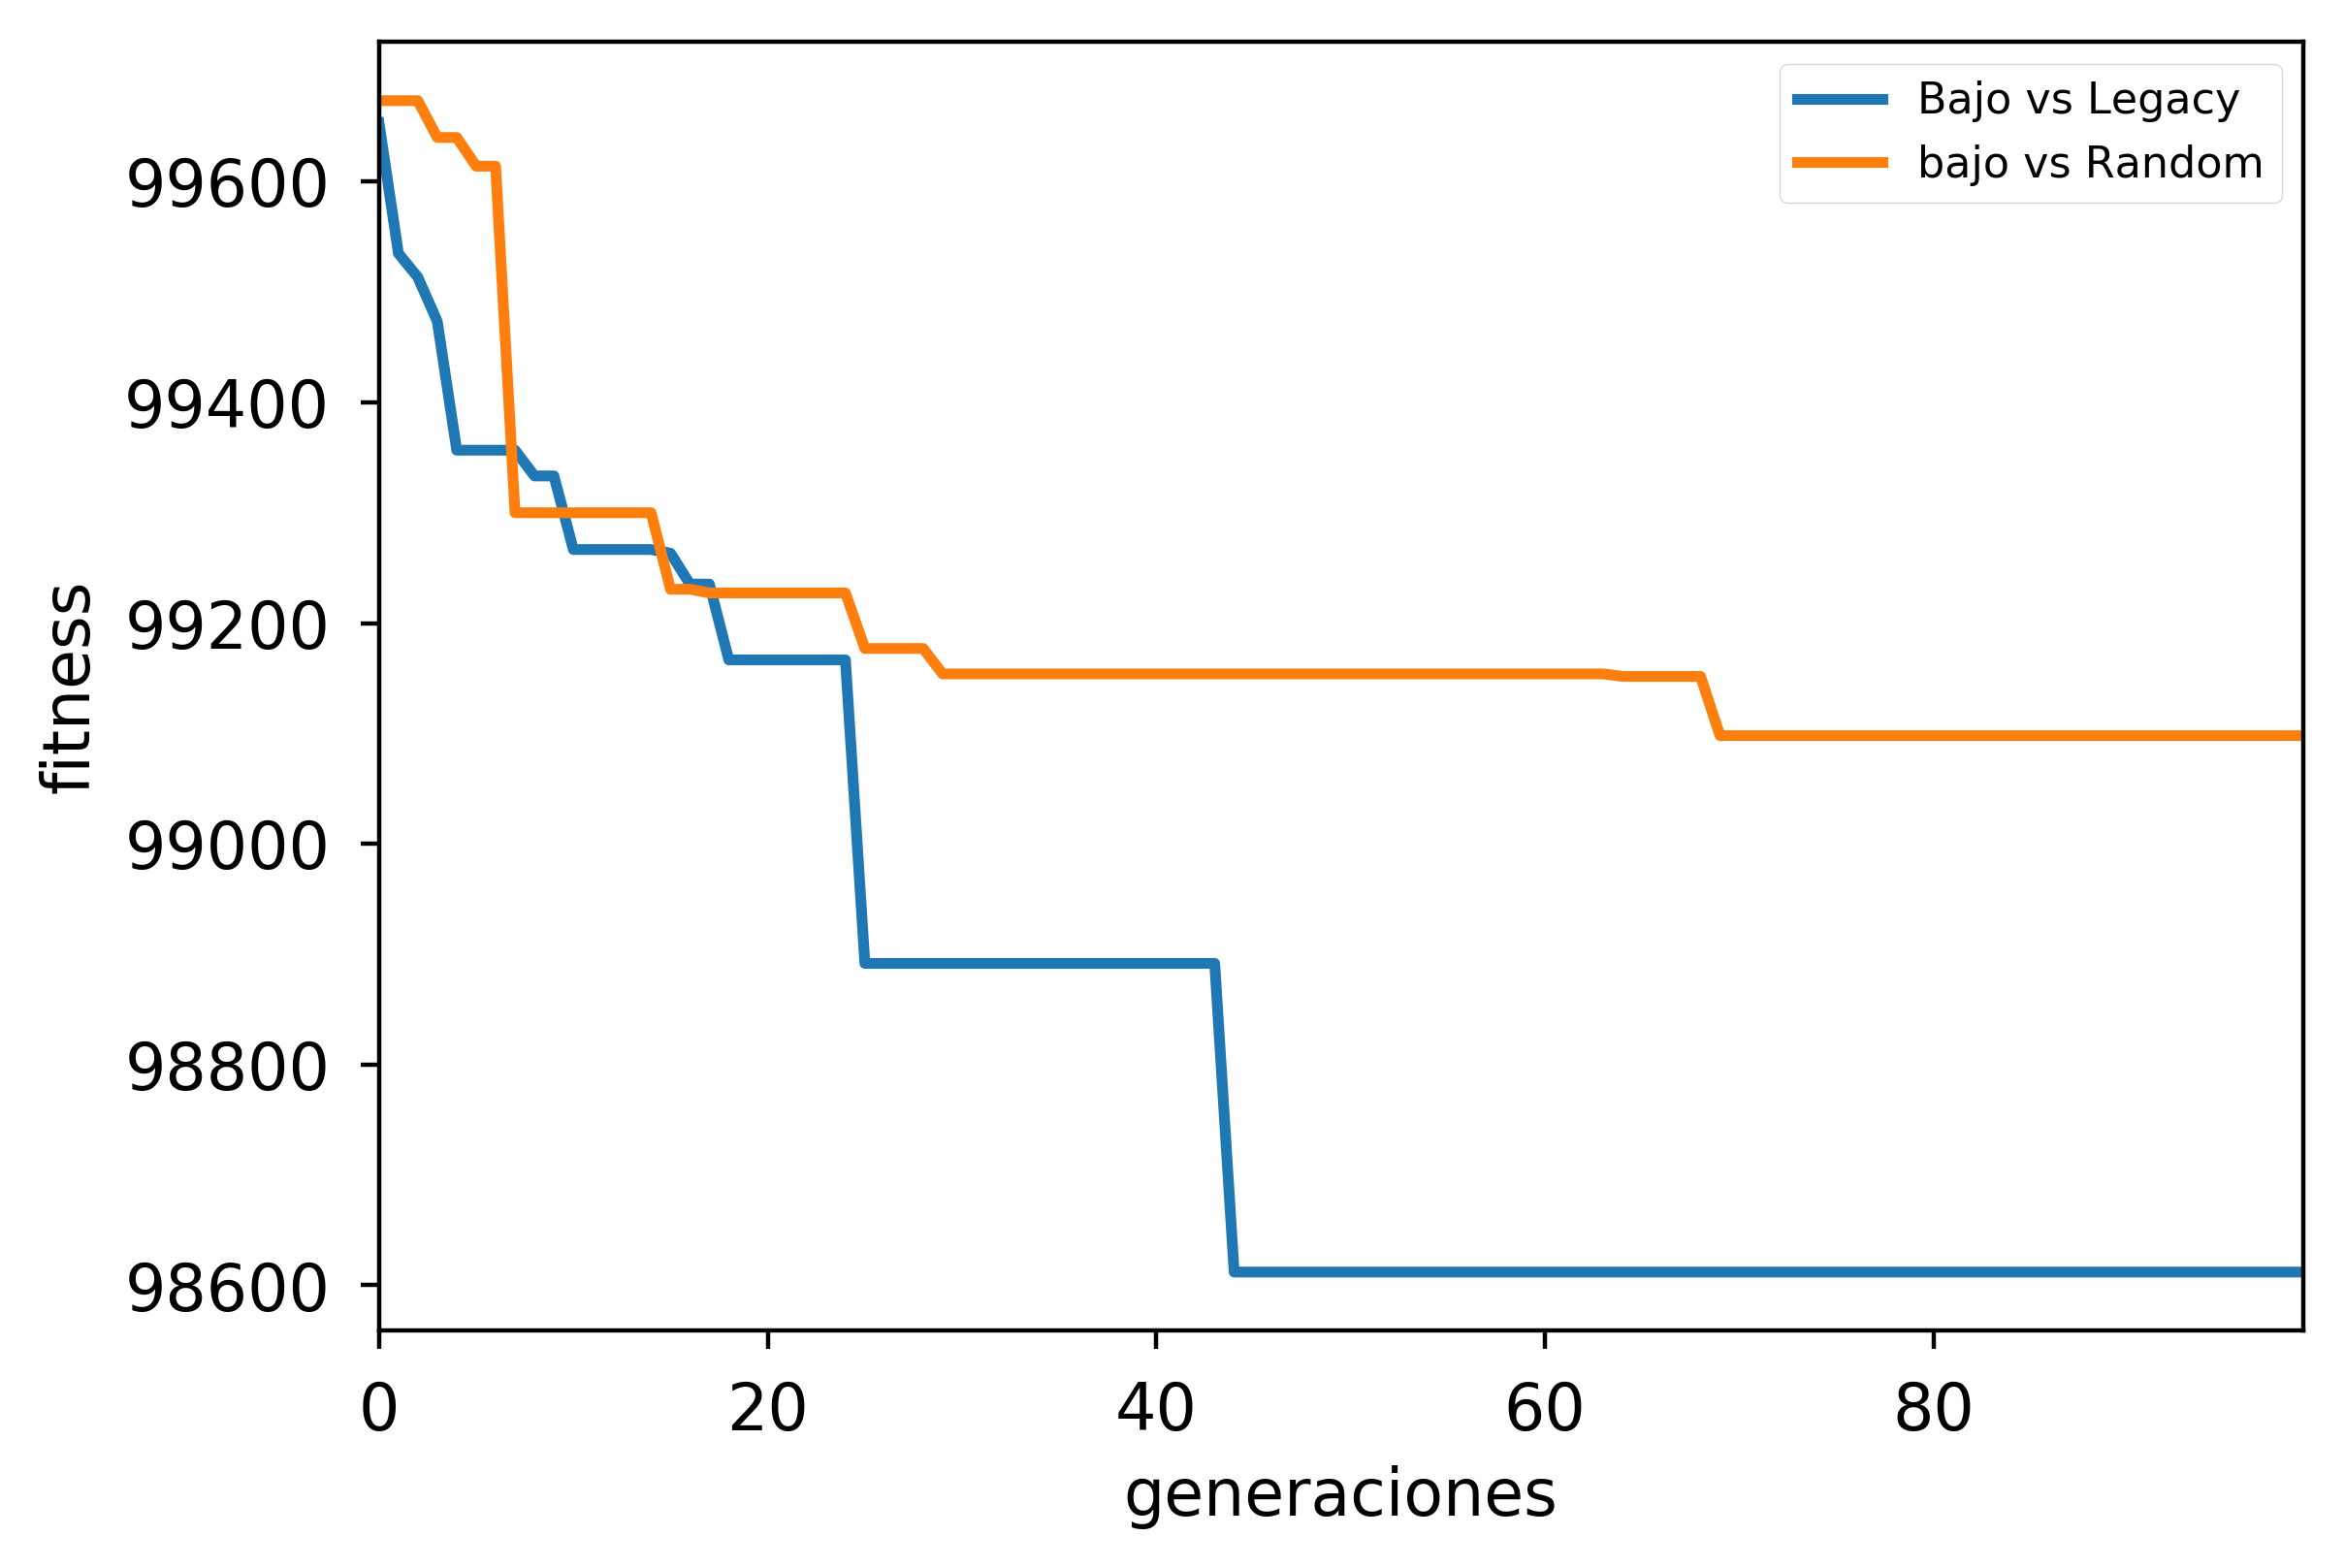
\includegraphics[width=0.8\textwidth]{grafica/low_level}
\end{figure}

Se obtuvieron las siguientes conclusiones a través de distintas ejecuciones:
\begin{itemize}
\item Los programas generados (fenotipo) son bastante largos debido a que hay muchos anidamientos de \texttt{if-else} que generan distintas acciones para determinados casos particulares. Esto es un resultado esperado al usar la gramática de bajo nivel.

\item Se obtienen malos resultados en cuanto a puntos obtenidos pero hay una gran convergencia de la población hacia el individuo óptimo actual.

\item El comportamiento del mejor individuo es siempre el mismo. Pac-Man va directamente a la esquina inferior izquierda del nivel y se queda quieto en cierto punto en el cual los fantasmas no le detectan, consiguiendo pasarse niveles porque el juego cada 4000 \textit{ticks} cambia de nivel inexorablemente y da una cierta cantidad de puntos al jugador. Este error del juego solo lo detecta hasta el nivel 3, nivel en el que es siempre eliminado por los fantasmas. A este comportamiento le hemos denominado bot ``Camper''.
\end{itemize}

\begin{lstlisting}[frame=single, breaklines=no, basicstyle=\fontsize{10}{11}\ttfamily, caption=Ejemplo de bot típico producido usando la gramática de bajo nivel entrenado contra Random Ghosts]
if (getDistanceToClosestNonEdibleGhostUpNE25) {
  if (getDistanceToClosestNonEdibleGhostLeftLE90) {
    moveRight
  } else {
    if (getDistanceToClosestJunctionLeftLE10) {
      if (getClosestEdibleGhostDistanceToClosestJunctionRightLT20) {
        if (getDistToClosestPowerPillUpLT30) {
          moveLeft
        } else {
          if (getDistanceToClosestNonEdibleGhostDownGT25) {
            moveRight
          } else {
            moveRight
          }
        }
      } else {
        if (getGeometricMeanDistanceToNonEdibleGhostsLT10) {
          moveLeft
        } else {
          if (getClosestJunctionExitsNumberLeftGT20) {
            if (getNumberOfActivePowerPillsGT90) {
              if (getClosestJunctionExitsNumberUpNE10) {
                moveLeft
              }
            }
          } else {
            moveUp
          }
        }
      }
    } else {
      if (getDistToClosestPowerPillDownNE15) {
        moveUp
      } else {
        if (getDistanceToClosestNonEdibleGhostUpGT60) {
          if (getClosestEdibleGhostDistanceToClosestJunctionRightLT60) {
            if (getDistToClosestPowerPillLeftGT5) {
              if (getNumberOfActivePowerPillsLE25) {
                if (getDistanceToClosestEdibleGhostGT25) {
                  moveLeft
                } else {
                  if (getDistanceToClosestEdibleGhostGE5) {
                    if (getClosestEdibleGhostDistanceToClosestJunctionRightGT10) {
                      if (getDistToClosestPowerPillUpGE50) {
                        moveRight
                      } else {
                        if (getDistanceToClosestJunctionUpEQ75) {
                          moveUp
                        } else {
                          if (getClosestJunctionExitsNumberLeftEQ20) {
                            moveDown
                          }
                        }
                      }
                    } else {
                      moveDown
                    }
                  } else {
                    moveDown
                  }
                }
              } else {
                moveUp
              }
            } else {
              moveUp
            }
          }
        }
      }
    }
  }
} else {
  if (getClosestEdibleGhostDistanceToClosestJunctionUpGT60) {
    if (getDistToClosestPowerPillLeftGE40) {
      moveDown
    } else {
      moveUp
    }
  } else {
    moveLeft
  }
}
\end{lstlisting}

\begin{lstlisting}[frame=single, breaklines=no, basicstyle=\fontsize{10}{11}\ttfamily, caption=Mejor individuo producido usando la gramática de bajo nivel evolucionado jugando contra Legacy Ghosts]
    if (getDistanceToClosestNonEdibleGhostRight LE 5) {
        moveDown
    }
    else {
        if (getDistanceToClosestEdibleGhostLeft LE 40) {
            moveUp
        }
        else {
            moveRight
        }
    }
\end{lstlisting}

\subsection{Gramática de medio nivel}
Con esta gramática de medio nivel intentamos obtener mejores resultados en puntos que los obtenidos con la gramática de bajo nivel. Hemos eliminado de la gramática los operadores de movimientos básicos (\texttt{moveUp, moveDown, ...}) debido a que han sido sustituidos por operadores más abstractos y de más alto nivel:
\begin{itemize}
\item \texttt{getDirectionTowardsClosestPill}: Devuelve el movimiento a efectuar (arriba, abajo, derecha, izquierda) para ir hacia la \textit{pill} más cercana al bot.

\item \texttt{getDirectionAwayFromClosestNonEdibleGhost}: Devuelve el movimiento a efectuar para alejarse (normalmente en dirección contraria al fantasma) del fantasma peligroso más cercano.

\item \texttt{getDirectionTowardsClosestEdibleGhost}: Devuelve el movimiento hacia el fantasma comestible más cercano.

\item \texttt{getDirectionTowardsClosestPowerPill}: Devuelve el movimiento hacia la \textit{power pill} más cercana.
\end{itemize}

Dado que estos operadores de acción disponen internamente de acceso al estado del juego hemos optado por prescindir de los operadores de obtención de información menos utilizados o que no son útiles en la gramática de medio nivel (como la distancia a la \textit{pill} más cercana al bot en dirección arriba). De este modo solo dispone de los operadores más útiles (y los que prácticamente siempre usa) y permite guiar la búsqueda más eficientemente.

\subsubsection{Notación BNF}
\begin{lstlisting}[frame=single, breaklines=no, basicstyle=\fontsize{10}{11}\ttfamily, caption=Gramática de medio nivel]
<grammar> ::= <selection-statement>

<selection-statement> ::= if( <condition> ){ <statement> } else{ <statement> }
                                        | if( <condition> ){ <statement> }

<statement> ::= <terminal-func>
              | <selection-statement>

<terminal-func> ::= getDirectionTowardsClosestPill
                  | getDirectionAwayFromClosestNonEdibleGhost
                  | getDirectionTowardsClosestEdibleGhost
                  | getDirectionTowardsClosestPowerPill
                  
<condition> ::= <number-func> <number-operator> <number>

<number-func> ::= getDistanceToClosestNonEdibleGhost
                | getDistanceToClosestEdibleGhost
                | getNumberOfActivePowerPills
                | getDistToClosestPill
                | getDistToClosestPowerPill
                | getGeometricMeanDistanceToNonEdibleGhosts
                | getGeometricMeanDistanceToEdibleGhosts

<number-operator> ::= EQ
                    | NE
                    | LT
                    | GT
                    | LE
                    | GE

<number> ::= 5 | 10 | 15 | 20 | 25 | 30 | 40 | 50 | 60 | 75 | 80 | 90
\end{lstlisting}

\subsubsection{Resultados}
\begin{figure}[H]
\centering
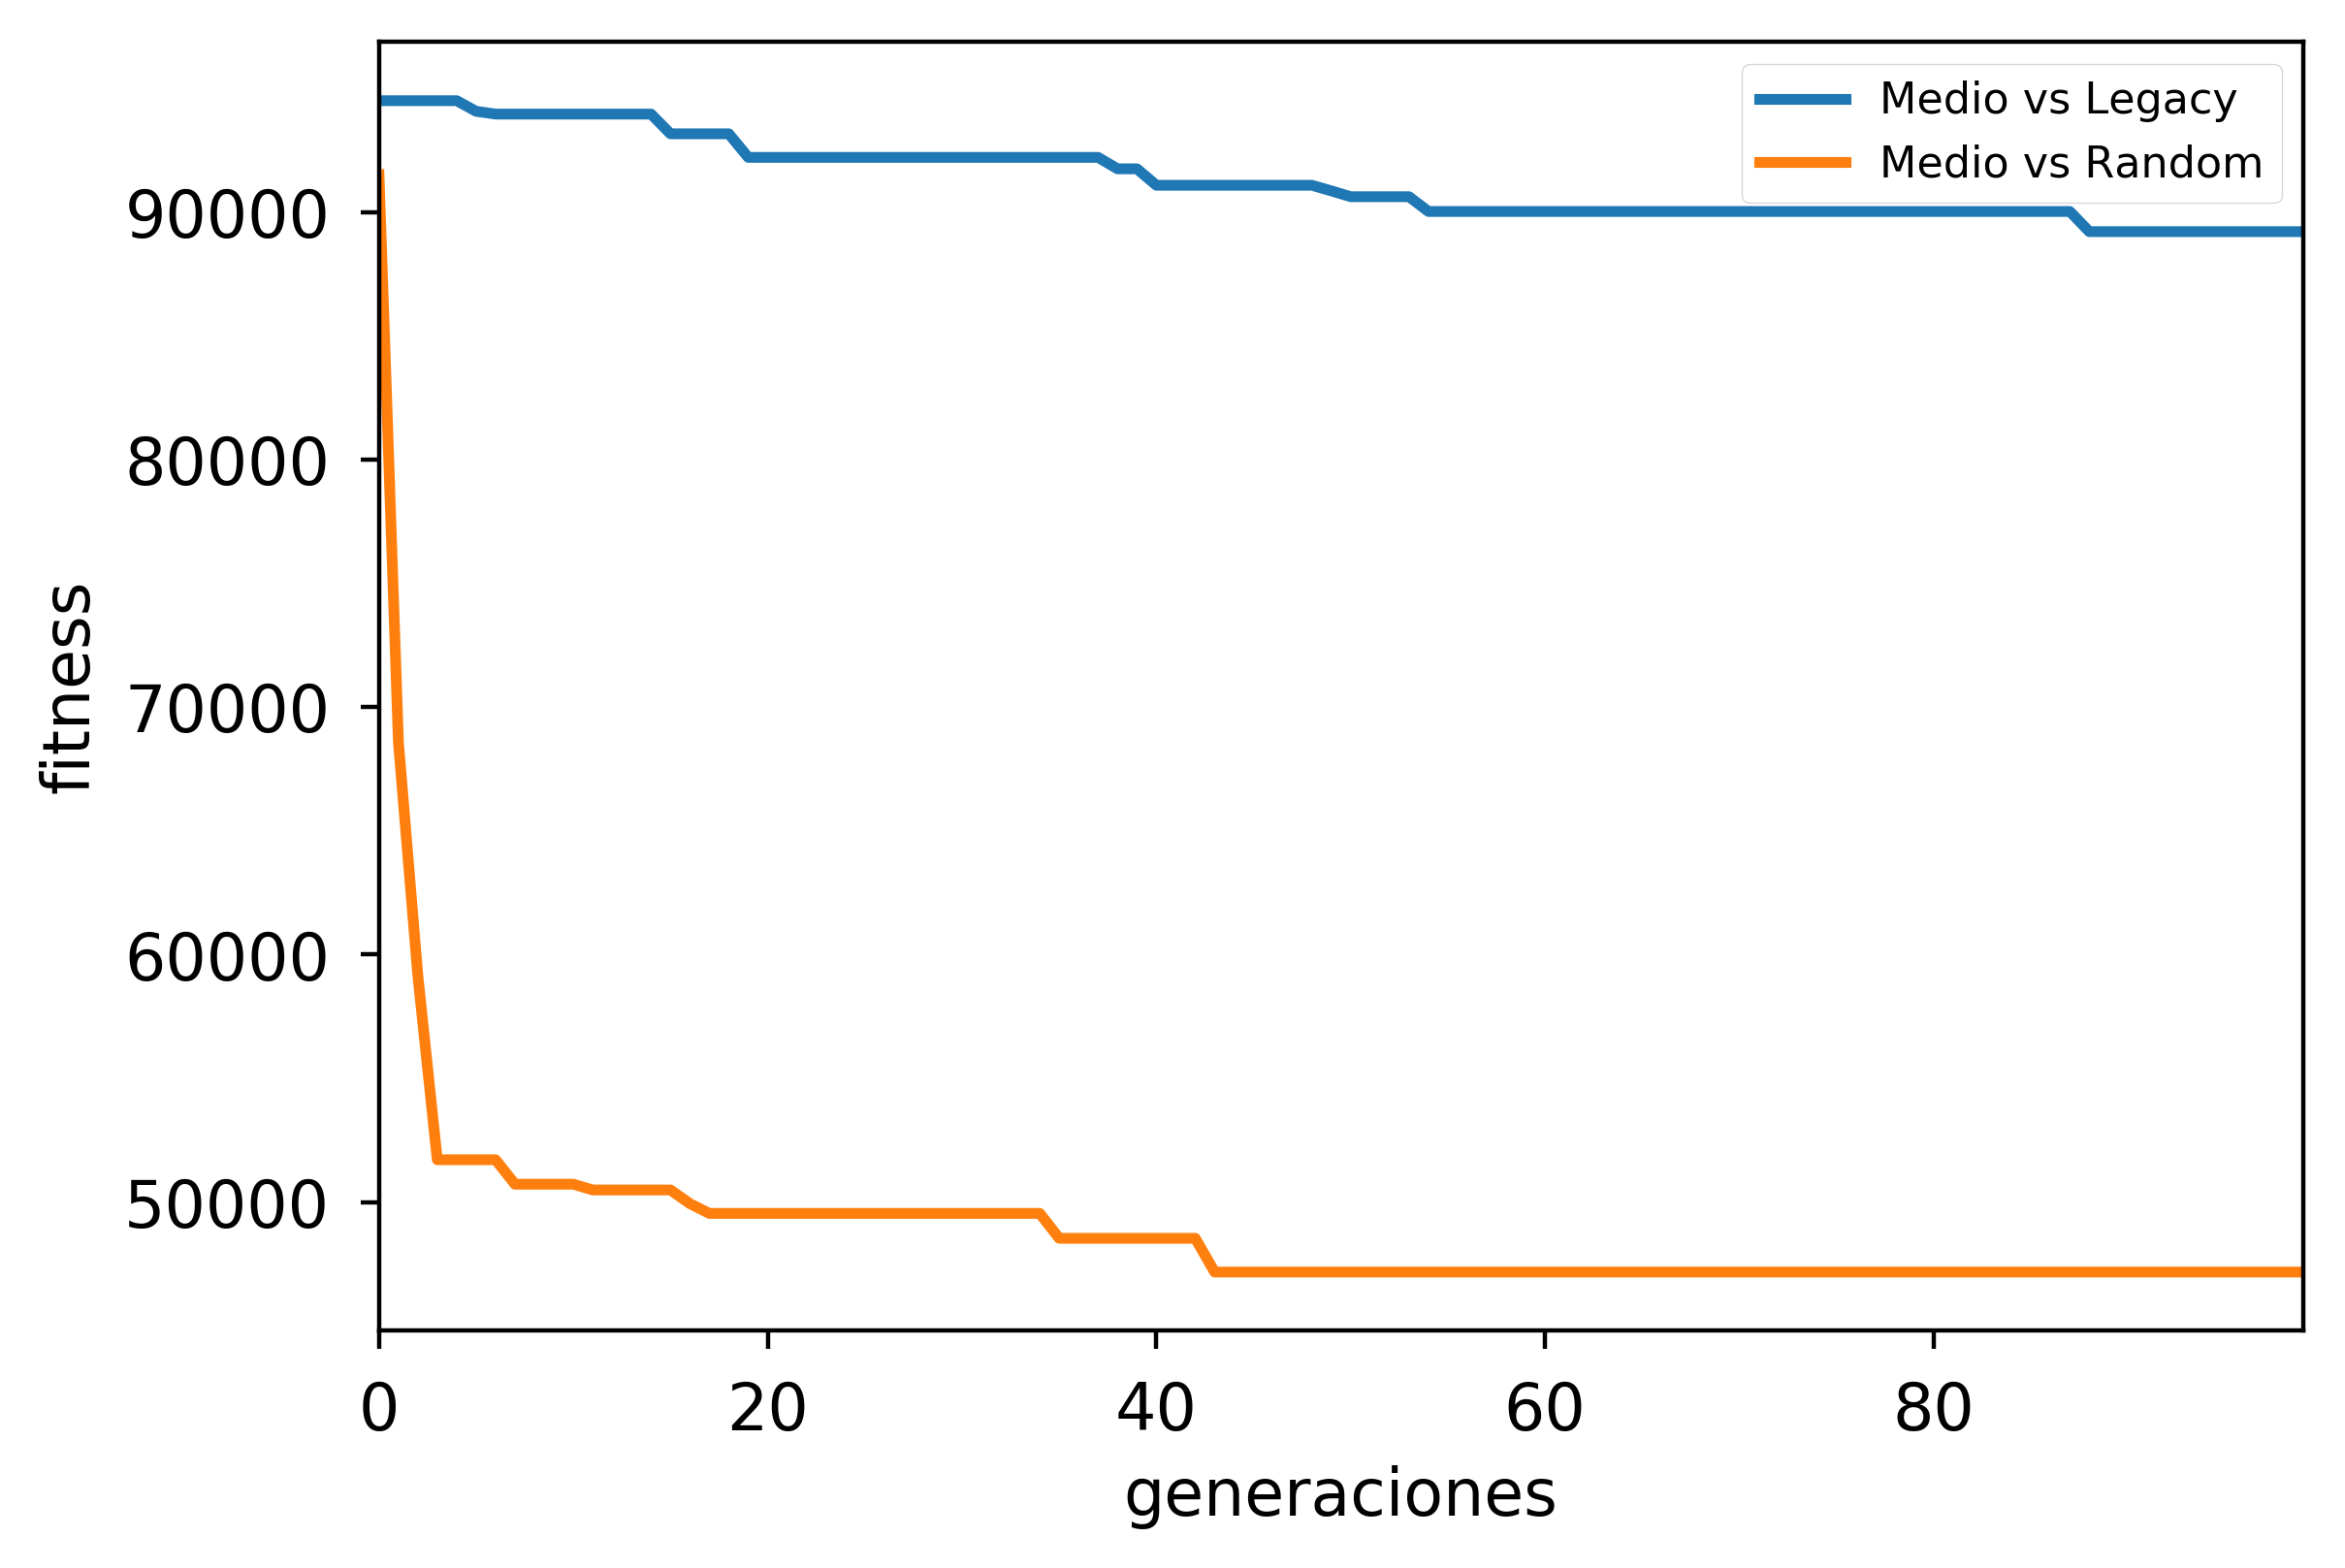
\includegraphics[width=0.8\textwidth]{grafica/medium_level}
\end{figure}

Las conclusiones obtenidas son:
\begin{itemize}
\item La velocidad de ejecución del algoritmo evolutivo ha sido significativamente más rápida que la de bajo nivel.

\item Los resultados obtenidos en puntos son bastante superiores a los obtenidos con la gramática de bajo nivel.

\item El código generado por el mejor individuo (fenotipo) es muy corto, generalmente consiste de un solo \textit{if-else} que contiene cada uno una única función.

\item Creemos que la longitud del código está directamente relacionada al comportamiento que poseen los mejores individuos y que es obtenido de forma recurrente. Al principio y si no hay fantasmas cercanos el bot solo realiza movimientos neutros (continuar en la misma dirección), quedándose atascado en una esquina del mismo modo que lo hace el bot ``Camper'' de la gramática de nivel bajo. Pero si un fantasma se acerca lo suficiente el bot pasa a un modo agresivo dirigiéndose a la \textit{power pill} más cercana, comiéndosela y cazando a tantos fantasmas como puede. Este comportamiento lo repite con todas las \textit{power pills} hasta que se queda sin ellas, pasando a un estado de movimiento neutral y siendo eliminado por los fantasmas sin pasar nunca del primer nivel del juego. Este comportamiento es debido a una característica del juego que provoca una explosión en la puntuación al comer fantasmas seguidos. Esto se debe a que durante el tiempo que dura el efecto de una \textit{power pill} cada fantasma comido da una serie de puntos, este valor es duplicado si se come otro fantasma y el nuevo valor es a su vez duplicado si otro fantasma es consumido. Esto permite obtener una gran cantidad de puntos provocando que el fitness de ese individuo destaque
\end{itemize}

Como se puede apreciar, la gramática de bajo nivel siempre lleva a un comportamiento de bot ``Camper'' y la gramática de medio nivel a un comportamiento de bot ``Cazador''. Estos comportamientos vienen dados principalmente por los puntos que se obtienen al jugar, por lo que investigamos el uso de una gramática de alto nivel y comparamos los resultados obtenidos con la gramática de medio nivel. Así mismo estudiamos distintas funciones \textit{fitness} y comprobamos si con estas nuevas funciones conseguimos mejores comportamientos.

\begin{lstlisting}[frame=single, breaklines=no, basicstyle=\fontsize{10}{11}\ttfamily, caption=Mejor individuo producido usando la gramática de medio nivel para evolucionar contra Random Ghosts.]
    if (getDistanceToClosestNonEdibleGhost > 10) {
        if (getDistanceToClosestNonEdibleGhost < 20) {
            getDirectionTowardsClosestPowerPill 
        }
        else {
            getDirectionTowardsClosestPill
        }
    }
    else {
        getDirectionAwayFromClosestNonEdibleGhost
    }
\end{lstlisting}

\begin{lstlisting}[frame=single, breaklines=no, basicstyle=\fontsize{10}{11}\ttfamily, caption=Mejor individuo producido usando la gramática de medio nivel para evolucionar contra Legacy Ghosts.]
    if (getDistanceToClosestNonEdibleGhost >= 5) {
        getDirectionTowardsClosestPill
    } else {
        getDirectionAwayFromClosestNonEdibleGhost
    }
\end{lstlisting}

\subsection{Gramática de alto nivel}
Tras los resultados obtenidos con las gramáticas anteriores, decidimos estudiar hasta qué punto sería posible mejorarlos mediante el empleo de una gramática de alto nivel, empleando  un número reducido de funciones de alto nivel, proporcionándole de esta forma conocimiento experto.

\subsubsection{Nuevas funciones de alto nivel}

\paragraph{escapeHL}
Genera un movimiento de huida hacia la \textit{power pill} mas cercana si puede alcanzarla antes que el fantasma más cercano. Si no llega a tiempo o bien no quedan \textit{power pill}s, genera un movimiento de huida del fantasma más cercano en la dirección que más le aleje de él.

\paragraph{attackHL}
Genera un movimiento hacia el fantasma más comible cercano siempre que este pueda ser alcanzado por otro fantasma no comible antes. Si no hay fantasmas comibles, genera un movimiento igual a la última dirección en la que se movió.

\paragraph{seekFoodHL}
Genera un movimiento hacia la \textit{pill} más cercana (o si no quedan \textit{pills}, la \textit{power pill} más cercana) siempre y cuando sea alcanzable por Pac-Man antes que por un fantasma. Si no llega a tiempo, mueve en la última dirección en la que lo hizo el turno anterior.

\subsubsection{Notación BNF}
\begin{lstlisting}[frame=single, breaklines=no, basicstyle=\fontsize{10}{11}\ttfamily, caption=Gramática de alto nivel.]
<grammar> ::= <selection-statement>

<selection-statement> ::= if( <condition> ){ <statement> } else{ <statement> }
                        | if( <condition> ){ <statement> }

<statement> ::= <terminal-func>
              | <selection-statement>

<terminal-func> ::= escapeHL
                  | attackHL
                  | seekFoodHL

<condition> ::= <number-func> <number-operator> <number>

<number-func> ::= getDistanceToClosestNonEdibleGhost
                | getDistanceToClosestEdibleGhost

<number-operator> ::= EQ
                    | NE
                    | LT
                    | GT
                    | LE
                    | GE

<number> ::= 5 | 10 | 15 | 20 | 25 | 30 | 40 | 50 | 60 | 75 | 80 | 90
\end{lstlisting}

\subsubsection{Resultados}
Debido al conocimiento experto que poseen las funciones, la gramática utilizada solo contiene como operadores de acción las tres funciones de alto nivel comentadas, dos operadores de obtención de información del tablero  (\texttt{getDistanceToClosestNonEdibleGhost} y \texttt{getDistanceToClosestEdibleGhost}) debido a que recurrentemente han sido las más utilizadas, el comportamiento de los mejores bots obtenidos con las gramáticas anteriores se basan únicamente en ellas para la toma de decisiones.
\begin{figure}[H]
\centering
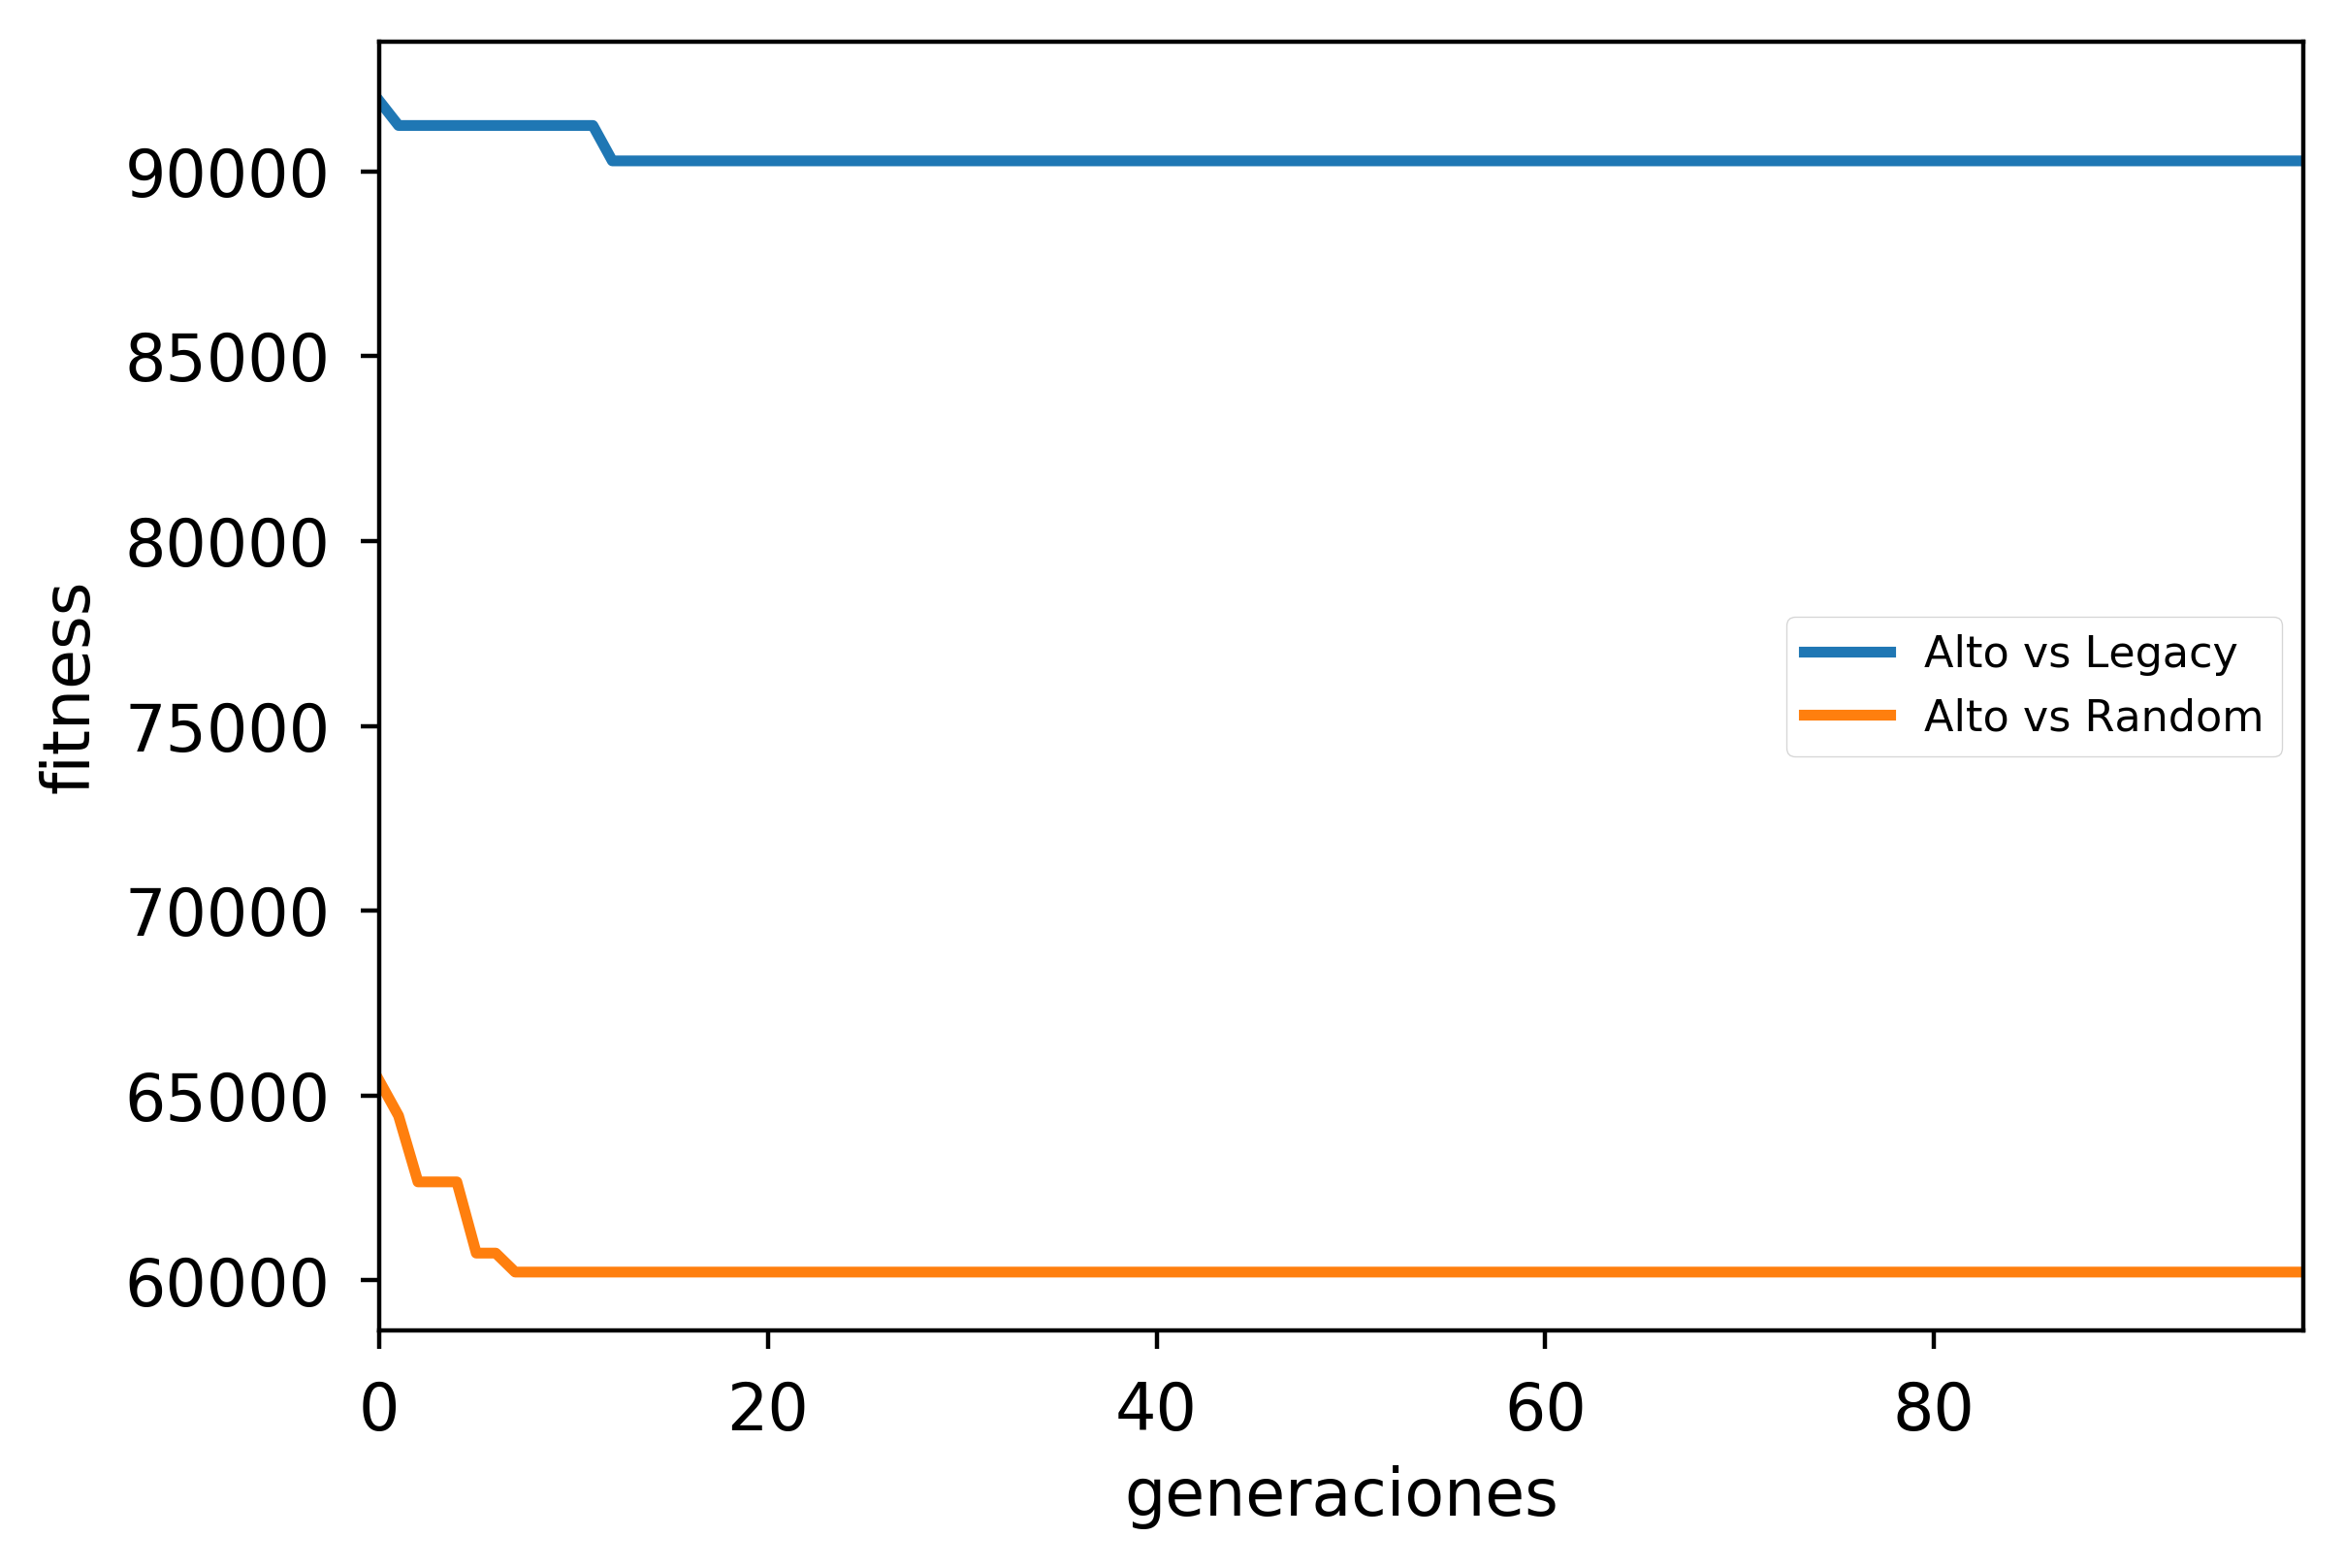
\includegraphics[width=0.8\textwidth]{grafica/high_level}
\end{figure}

Las conclusiones obtenidas al evolucionar el bot usando esta gramática fueron:
\begin{itemize}
\item La velocidad de ejecución del algoritmo es aún más rápida que con la gramática de medio nivel.

\item El código generado habitualmente se parece mucho al obtenido mediante la gramática de medio nivel: Un \textit{if-else} con una inecuación numérica que generalmente tiene en cuenta el fantasma más cercano. La más notable diferencia es que las acciones de medio nivel como \texttt{getDirectionAwayFromClosestNonEdibleGhost}, se ven sustituidas por su correspondiente directa de alto nivel, como \texttt{escapeHL}.
\begin{lstlisting}[frame=single, breaklines=no, basicstyle=\fontsize{10}{11}\ttfamily, caption=Código del mejor individuo obtenido en una población evolucionada con la gramática de medio nivel.]
    if (getDistanceToClosestNonEdibleGhost >= 5) {
        getDirectionTowardsClosestPill
    } else {
        getDirectionAwayFromClosestNonEdibleGhost
    }
\end{lstlisting}

\begin{lstlisting}[frame=single, breaklines=no, basicstyle=\fontsize{10}{11}\ttfamily, caption=Código del mejor individuo obtenido en una población evolucionada con la gramática de alto nivel.]
    if (getDistanceToClosestNonEdibleGhost <= 5) {
        escapeHL
    } else {
        seekFoodHL
    }
\end{lstlisting}

\item Obtiene buenos resultados muy rápidamente comparada con la gramática de medio nivel (Figura~\ref{grafica:comparacion-todas}). Esto se debe probablemente al reducido espacio de búsqueda de soluciones al ser una gramática tan compacta. Sin embargo y como se analizó en (citar paper),  la evolución utilizando la gramática de alto nivel se estanca en un óptimo local y es superada por la de medio nivel que obtiene mejores resultados, como se puede apreciar en la Figura~\ref{grafica:comparacion-todas}. La de medio nivel consigue algunos puntos más en promedio con 100 generaciones.
\end{itemize}

Todo esto nos indica que para tareas en las que es importante obtener buenos resultados de forma rápida, conviene favorecer gramáticas de alto nivel, mientras que si buscamos los mejores resultados posibles a cambio de un tiempo de evolución largo, conviene usar gramáticas de medio nivel.

\begin{lstlisting}[frame=single, breaklines=no, basicstyle=\fontsize{10}{11}\ttfamily, caption=Ejemplo de bot producido al evolucionar usando la gramática de alto nivel (mismo resultado entrenando tanto contra Random Ghosts como Legacy Ghosts).]
    if (getDistanceToClosestNonEdibleGhost <= 5) {
        escapeHL
    } else {
        seekFoodHL
    }
\end{lstlisting}

\subsection{Comparativa gráfica de niveles}
\begin{figure}[H]
\centering
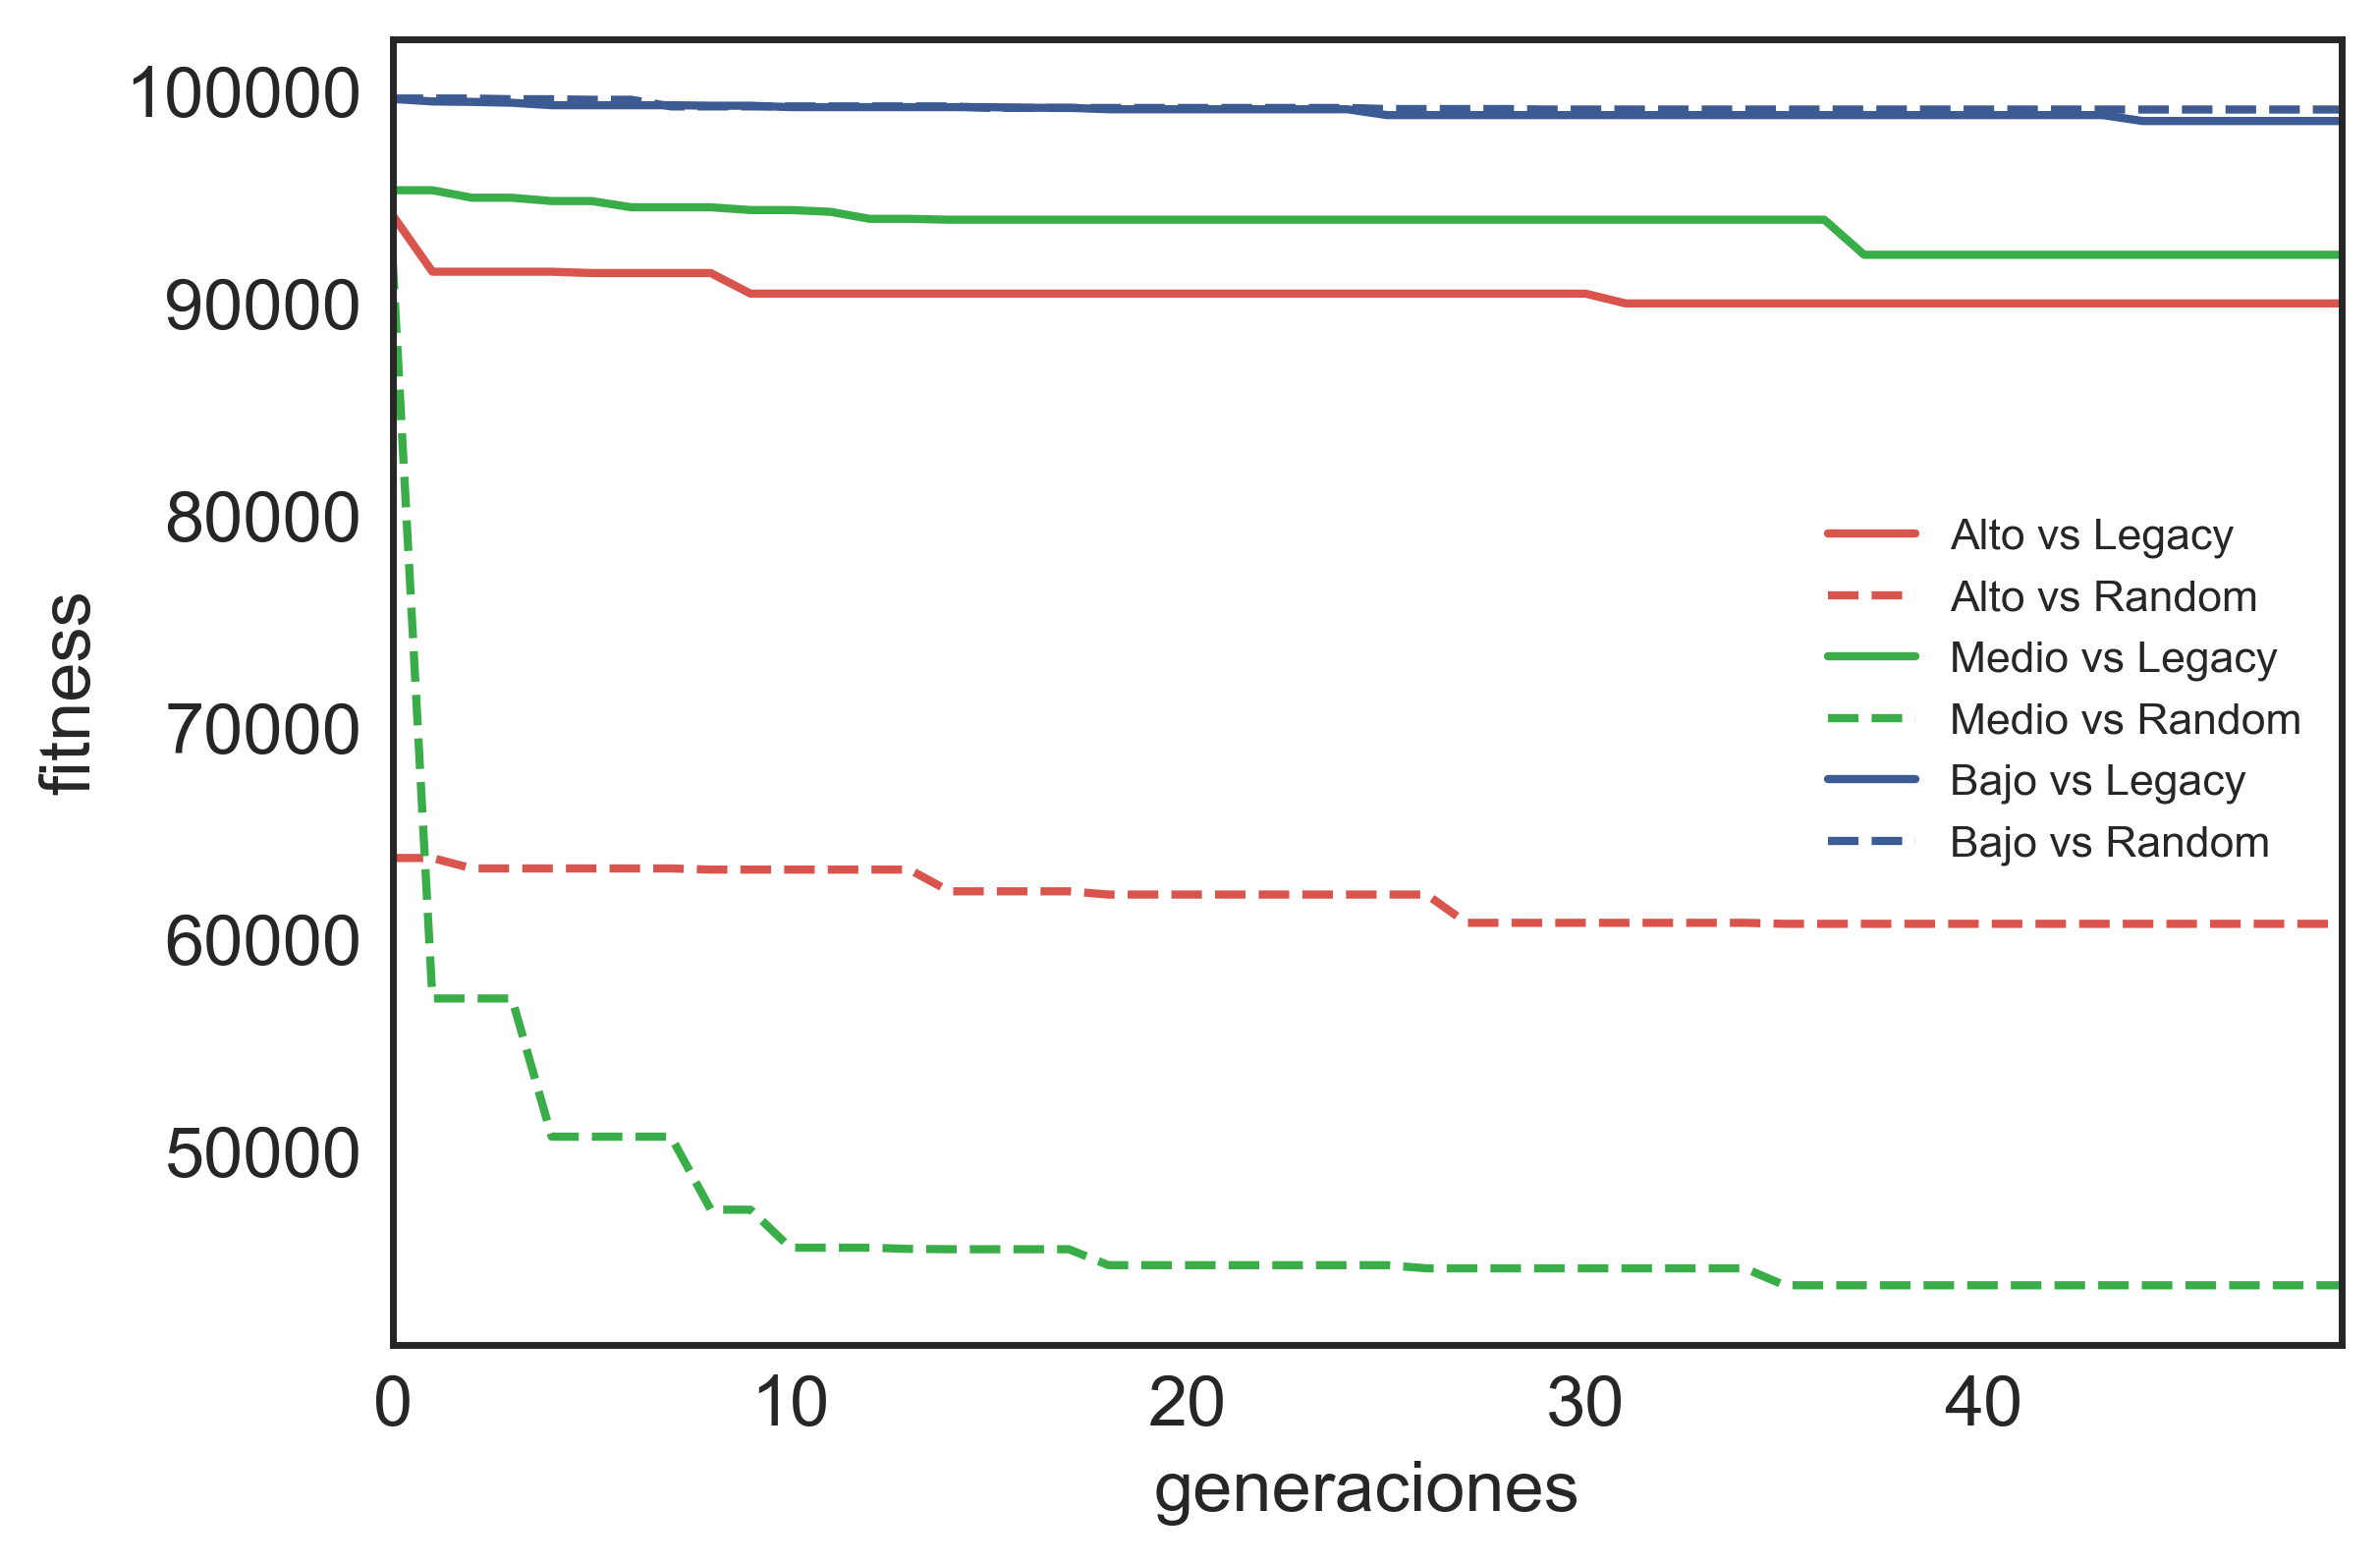
\includegraphics[width=0.8\textwidth]{grafica/all_fitnesses}
\label{grafica:comparacion-todas}
\caption{Gráfica de comparación de la evolución de una misma población usando las gramáticas de bajo, medio y alto nivel para dos controladores de fantasmas distintos (menos es mejor).}
\end{figure}

\section{Estudios, optimizaciones y mejoras}
Llegados a este punto nos planteamos realizar varios estudios relativos al rendimiento del algoritmo evolutivo, basadas en inquietudes fundadas en numerosos artículos científicos, para verificar que no se estaba produciendo ninguna inconsistencia dentro del entrenamiento de dicho algoritmo evolutivo. Además, también realizamos una serie de optimizaciones sobre funciones ya existentes en JECO, con el fin de reducir lo máximo posible el tiempo de ejecución y retocar algunas opciones por defecto del framework evolutivo para mejorar los resultados.

\subsection{Estudio de la presión selectiva}
Una de los factores que consideramos de importancia dentro de nuestro algoritmo evolutivo es la conservación de diversidad dentro de nuestra población y tratar de evitar el estancamiento en óptimos locales, la convergencia prematura y la evolución en avalancha producidas por la falta de ésta diversidad. Para ello hemos decidido evaluar cuál es la presión selectiva durante la ejecución, siendo esta la frecuencia con que es seleccionado el mejor individuo frente al resto. Esto se calcula en problemas de maximización mediante la siguiente fórmula
\begin{equation}
\textrm{Presión selectiva} = \frac{\textrm{fitness mejor}}{\textrm{fitness promedio}}
\end{equation}
En nuestro caso, al ser el nuestro un problema de minimización ($100000 - score$) empleamos:
\begin{equation}
\textrm{Presión selectiva} = \frac{\textrm{fitness promedio}}{\textrm{fitness mejor}}
\end{equation}

Habitualmente se recomienda emplear una presión selectiva en torno a $1.5$ \cite{whitley1989genitor}, mientras que nosotros a partir de mediciones hemos comprobado que empleamos una de aproximadamente $1.7$. No obstante, cada vez que se produce una mejora del mejor fitness  se produce un aumento proporcional en la presión selectiva, volviéndose a equilibrar al adaptarse el fitness promedio a esta mejora. No obstante, dicho aumento de la presión selectiva es despreciable.
 
Concluimos que tenemos una presión selectiva adecuada y por tanto no requerimos la implementación de ningún sistema de escalado del fitness de los individuos para mantener una conservación de diversidad.
\begin{figure}[H]
\centering
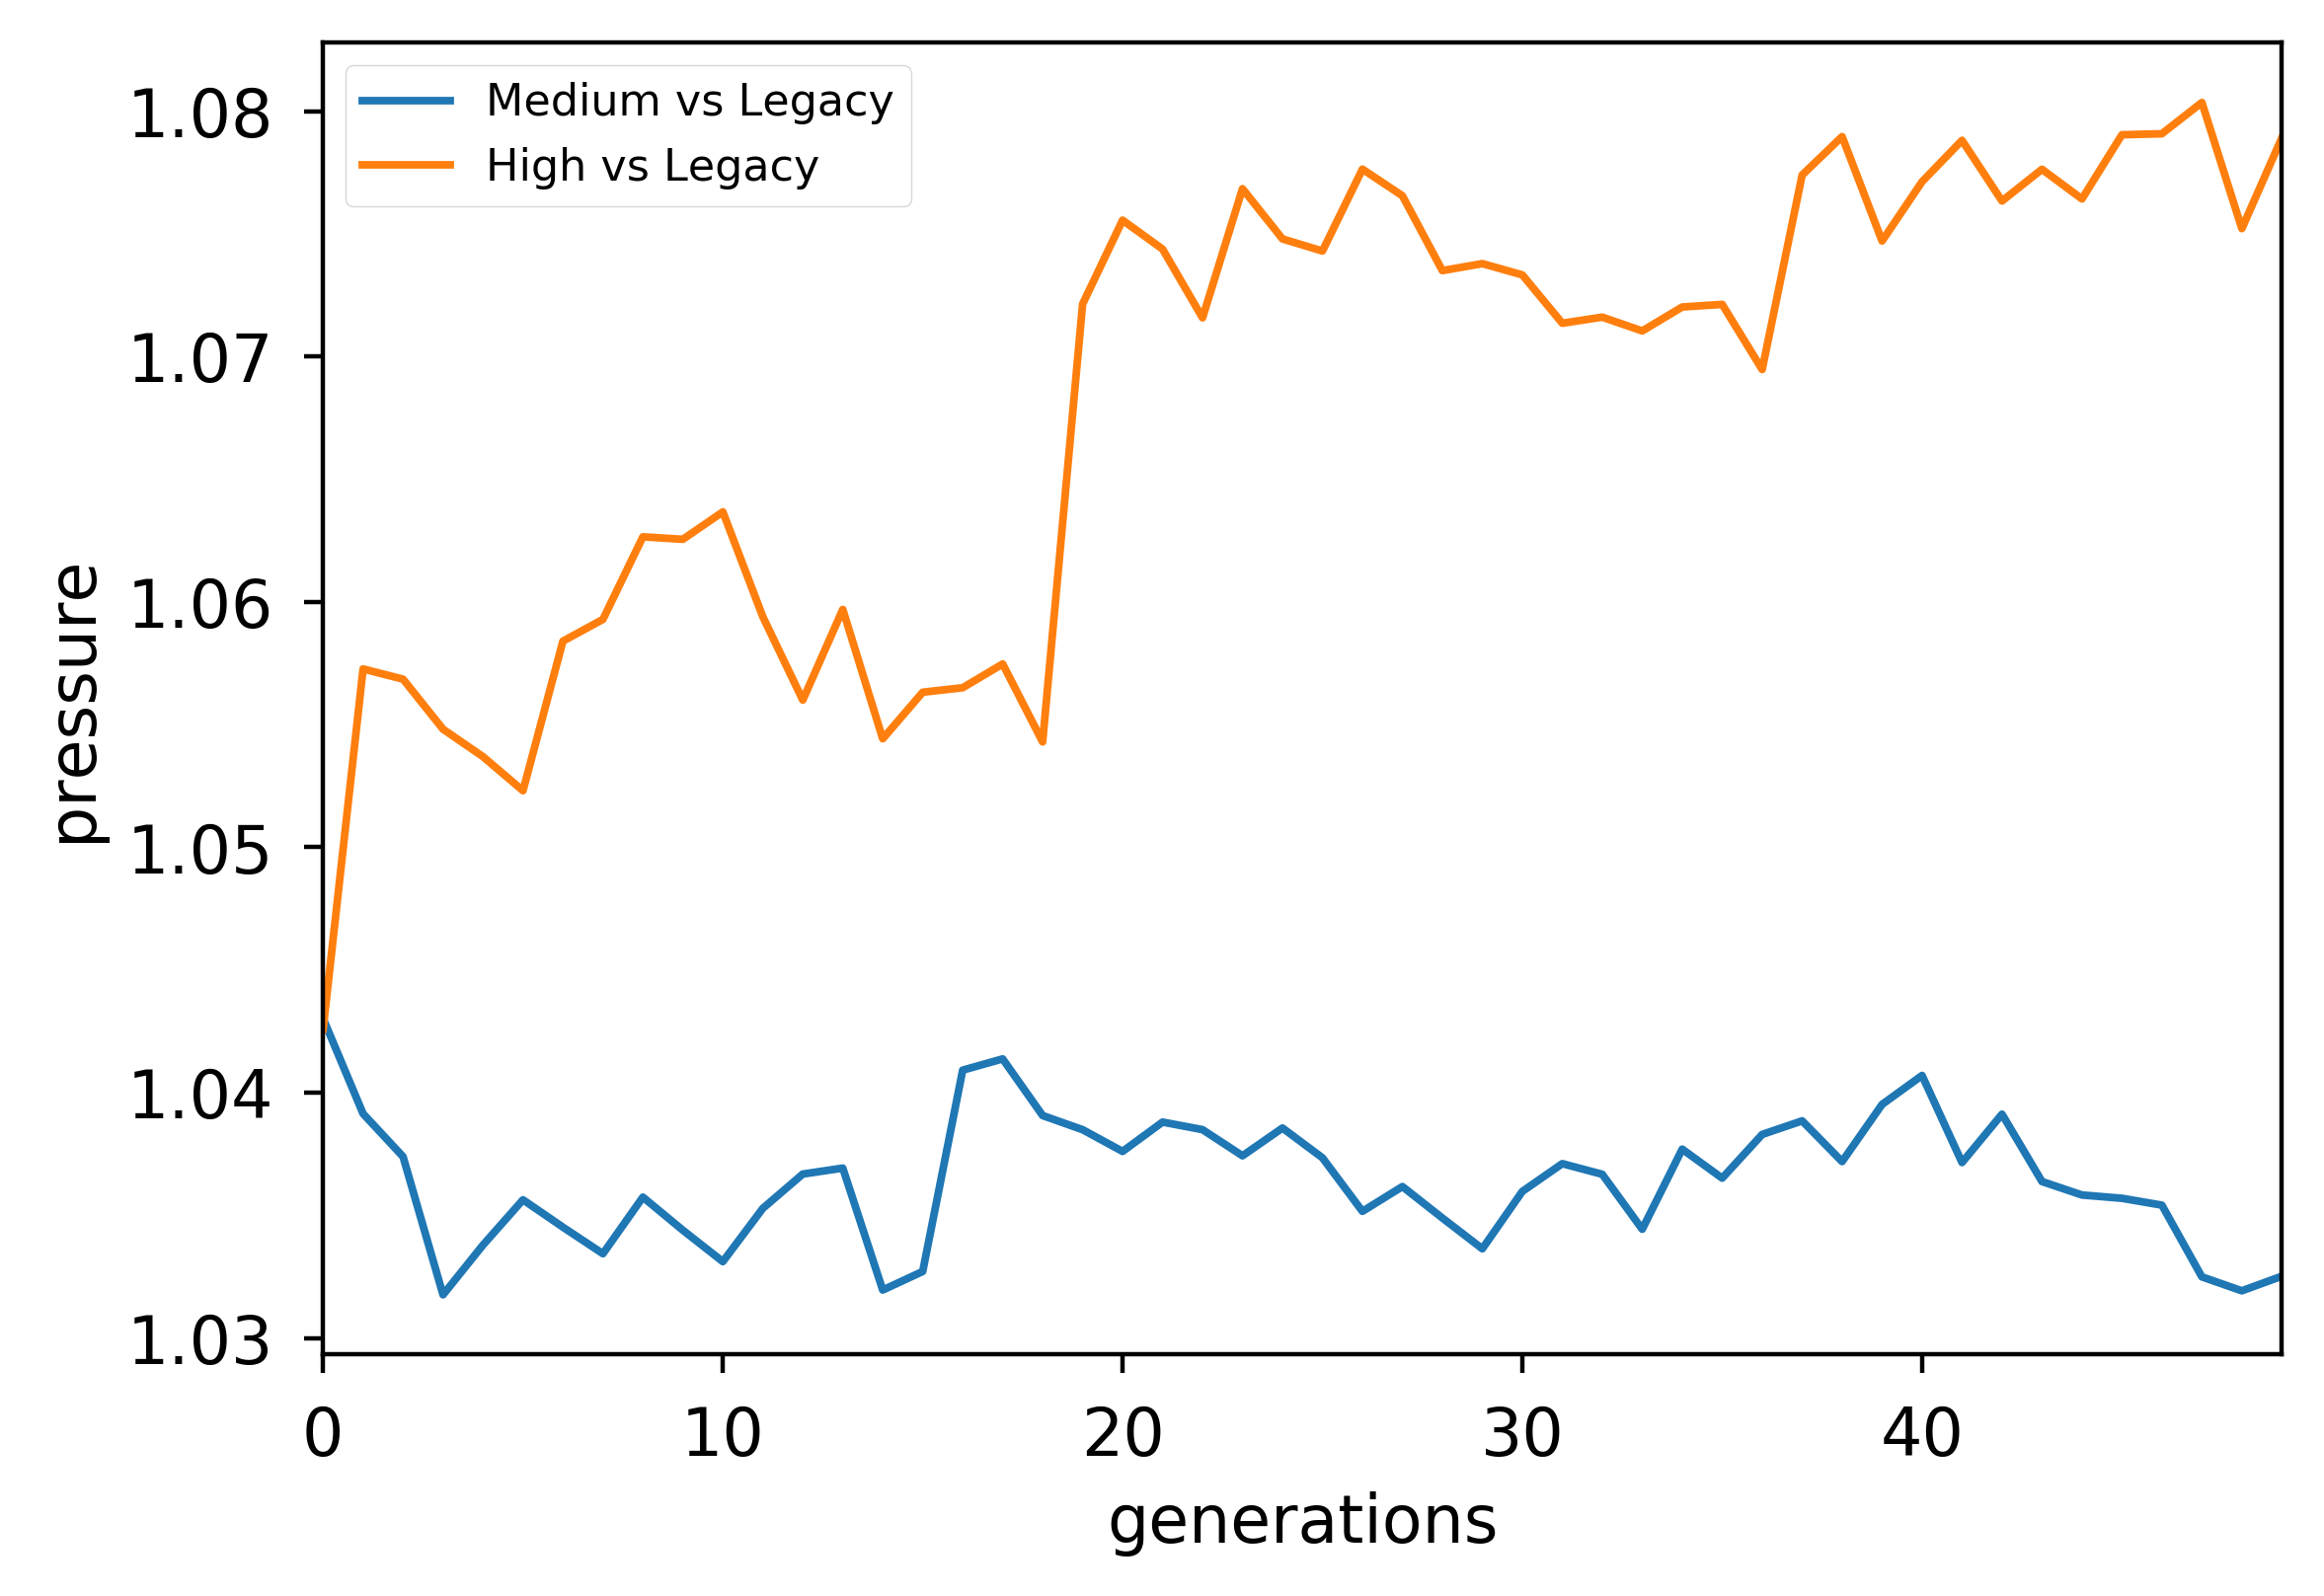
\includegraphics[width=0.8\textwidth]{grafica/presion-selectiva-detalle}
\caption{Vista en detalle  de la presión selectiva.}
\end{figure}

\begin{figure}[H]
\centering
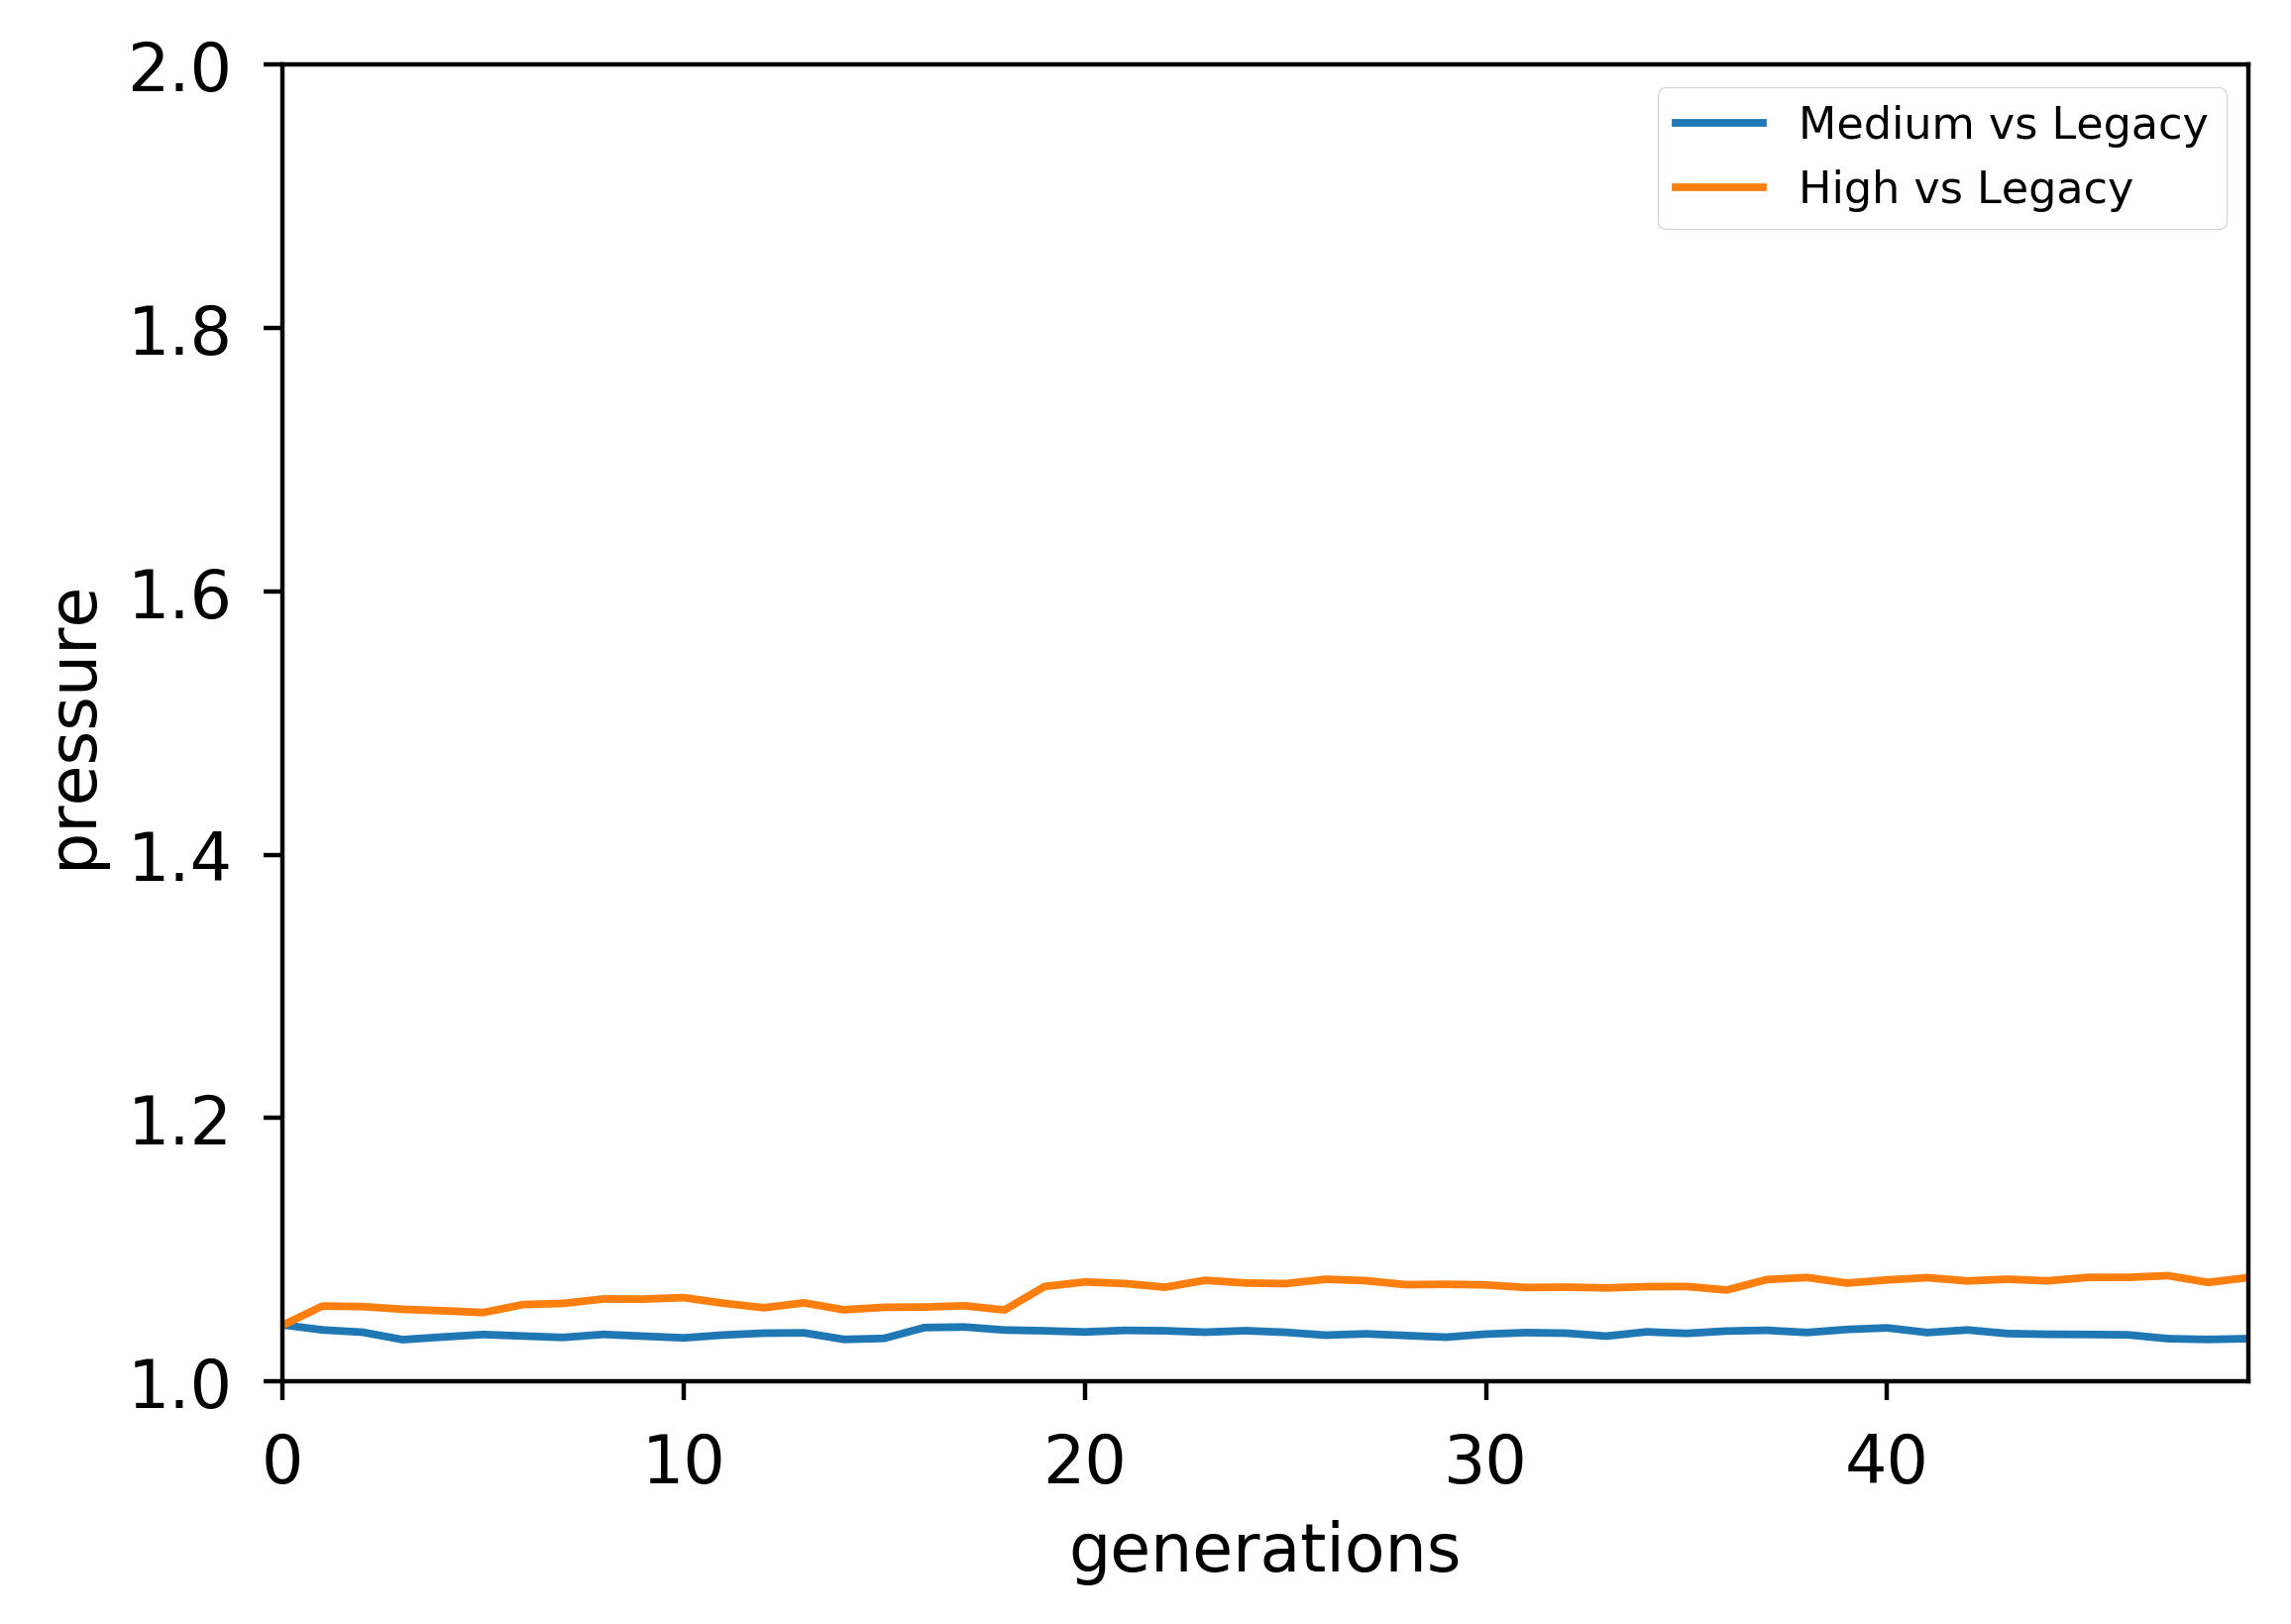
\includegraphics[width=0.8\textwidth]{grafica/presion-selectiva-general}
\caption{Vista global de la presión selectiva.}
\end{figure}

Además, tras un estudio en profundidad de nuestros operadores de selección hemos comprobado que todos (Torneo Binario, Torneo Binario NSGA y Torneo n-ario) emplean alguna modificación del operador de torneo, siendo este independiente al valor de la presión selectiva. Esto es así porque estos operadores no tienen en cuenta comparaciones entre fitness relativos (por ejemplo seleccionar proporcionalmente más veces los individuos con mejor fitness) sino comparaciones directas (seleccionar el individuo con mejor fitness entre varios elegidos de forma completamente aleatoria).

\subsection{Cruce LHS}
Antes de proceder con el estudio de nuevas funciones de \textit{fitness} decidimos comprobar si la razón por la que se producían programas tan cortos en las gramáticas de medio y alto nivel era por culpa del operador de cruce utilizado.

El operador de cruce monopunto usado en Gramáticas Evolutivas tiene el problema de generar mucho ruido en la población porque al cruzar los dos genotipos el nuevo hijo no suele guardar ninguna relación con los padres dada la forma en que se genera el fenotipo. Visto de otra forma, el cruce no copia un trozo de código de un individuo en el código del otro individuo, sino que lo altera desestructuradamente.

Para resolver este problema se implementa el cruce LHS que intenta solventar este problema. El cruce LHS, al igual que el monopunto, elige un punto aleatorio del genotipo pero en vez de cruzar la parte del genotipo restante a partir de ese punto lo que hace es ver cuántos codones expanden el símbolo no terminal marcado por el punto de cruce. Una vez visto cuántos codones componen la derivación total de dicho símbolo estos se insertan en la posición del punto de corte en el otro individuo, donde también se ha realizado el mismo proceso.

Este nuevo cruce produce ligeramente mejores resultados y menos ruido en la población pero tampoco se aprecia una gran mejoría en general. Aún así se convierte en el principal cruce que utilizamos en adelante.

\subsection{Estudio de uso de codones}
Durante la implementación del cruce LHS hicimos un estudio del número de codones utilizado en cada individuo para generar el fenotipo. El estudio lo hacemos con individuos de 100 y 50 codones permitiendo hacer \textit{wrapping}\footnote{El Wrapping se produce cuando se han procesado todos los codones del genotipo y aún no se ha llegado a procesar todos los símbolos no terminales dejando el fenotipo incompleto por lo que se sigue expandiendo los símbolos sin procesar usando nuevamente los codones del principio del genotipo.} 3 veces.  Los resultados obtenidos son los siguientes:
\begin{figure}[H]
\centering
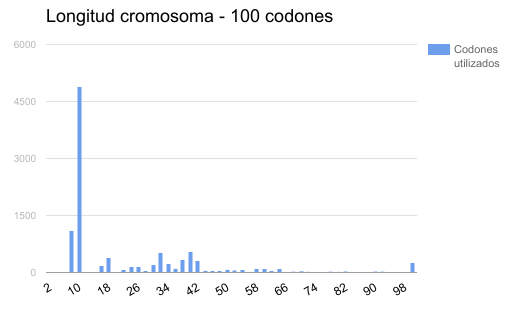
\includegraphics[width=0.8\textwidth]{grafica/codones-100}
\end{figure}

\begin{table}[H]
\centering
\begin{tabular}{ccccc}
\hline
\textbf{Media} & \textbf{Wrappings} & \textbf{Moda} & \textbf{Mediana} & \textbf{Desviación  est.} \\ \hline
23.9           & 331                & 10            & 10               & 21.7                      \\ \hline
\end{tabular}
\end{table}

\begin{figure}[H]
\centering
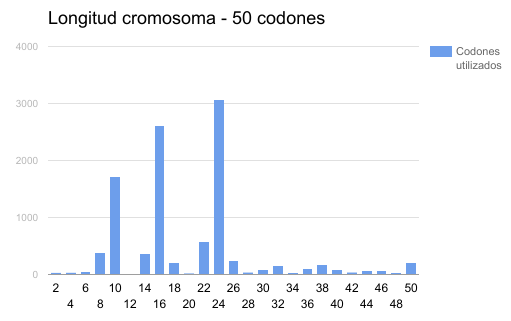
\includegraphics[width=0.8\textwidth]{grafica/codones-50}
\end{figure}

\begin{table}[H]
\centering
\begin{tabular}{ccccc}
\hline
\textbf{Media} & \textbf{Wrappings} & \textbf{Moda} & \textbf{Mediana} & \textbf{Desviación  est.} \\ \hline
20           & 375                & 24            & 18               & 9                      \\ \hline
\end{tabular}
\end{table}

Como se puede ver, cuando se usan longitudes de 100 codones los fenotipos se generan en su mayoría usando solo diez codones, lo que implica programas muy cortos y que la mayoría de las mutaciones y cruces sobre ellos no tienen efecto dado que se producen en el 90\% de los codones del genotipo que no se usan.

En cambio, con una longitud de 50 codones los individuos suelen generar individuos más largos, usando 25, 16 y 10 codones normalmente. Lo que sugiere que longitudes más pequeñas de cromosomas implican programas más largos a los que una mutación o un cruce los afecta en mayor medida y que pueden llegar a generar mejores resultados.

Para comprobar esto realizamos un banco de pruebas donde comprobar si es verdad que longitudes de cromosomas más cortas producen mejores resultados. Evolucionamos varias poblaciones idénticas pero variando en cada una la longitud de sus cromosomas, usando valores de 10 a 100 incrementados de diez en diez.

Los resultados obtenidos de este banco de pruebas no aportaron nada dado que los resultados y longitudes de fenotipos en las poblaciones con longitudes entre 40 y 100 eran prácticamente iguales, por lo que concluimos que la longitud del cromosoma no tiene mucha relación con los resultados obtenidos.

\subsection{Estudio de funciones fitness}
Como ya hemos visto, las gramáticas de bajo y medio nivel producen comportamientos demasiado específicos e incluso indeseados pero que consiguen muchos puntos. Hemos decidido probar nuevas funciones y ver el comportamiento obtenido por el bot. Para estas pruebas utilizaremos la última versión de la  gramática de nivel medio y con los mismos valores y operadores para los operadores de cruce, mutación, etc (Apartado~\ref{sec:params}).
\begin{itemize}
\item \textit{Puntuación \{1000000 - puntuación media\}}: Es la función de \textit{fitness} que se utiliza de forma genérica. Puntúa a los individuos por la puntuación media obtenida al evaluarlos, siendo los mejores individuos aquellos que obtengan mayor puntuación media.

Esta función se estanca siempre en un óptimo local produciendo el bot ``cazador'' el cual solo busca comerse el mayor número de fantasmas dado que esta acción produce una gran cantidad de puntos, pero una vez acabadas las \textit{power pill} realiza movimientos neutrales o come la \textit{pill} más cercana sin importarle la posición de los fantasmas, por lo que es eliminado por los fantasmas y no es habitual que complete el nivel uno.

\begin{lstlisting}[frame=single, breaklines=no, basicstyle=\fontsize{10}{11}\ttfamily, caption=Mejor individuo obtenido mediante esta función fitness.]
    if( getDistanceToClosestEdibleGhost <= 20 ){ 
        getDirectionTowardsClosestPowerPill
    }
\end{lstlisting}

\item \textit{Pills \{1000 - media de pills consumidas\}}: \textit{Fitness} que tiene como objetivo comer el máximo número de \textit{pills} posibles, sin importar la puntuación obtenida ni el nivel, aunque este último está directamente relacionado con comer \textit{pills}. Al mejor individuo que suele producir le hemos denominado bot ``Glotón''.

Este bot se centra únicamente en comer \textit{pills} normales pero, si se siente amenazado por un fantasma cercano, se dirige hacia una \textit{power pill}, la consume y sigue comiendo \textit{pills} normales (pero no caza a los fantasmas). Cuando no dispone de más \textit{power pills} a las que dirigirse y un fantasma se acerca, este sigue comiendo \textit{pills} normales y es consumido por los fantasmas. Este bot suele perder en el nivel dos o en el nivel uno cuando quedan pocas \textit{pills} por comer. El código producido es el antónimo del producido por el \textit{fitness} de \textit{Puntuación}.

\begin{lstlisting}[frame=single, breaklines=no, basicstyle=\fontsize{10}{11}\ttfamily, caption=Mejor individuo obtenido mediante esta función fitness.]
    if( getDistanceToClosestNonEdibleGhost >= 25 ){ 
        getDirectionTowardsClosestPill
    }
    else{ 
        getDirectionTowardsClosestPowerPill
    }
\end{lstlisting}

\item \textit{Niveles \{10 - máximo nivel alcanzado\}}: El objetivo de este \textit{fitness} es pasarse el mayor número de niveles sin importar la puntuación, las \textit{pills} comidas, el tiempo utilizado, etc por lo que los mejores individuos son los que han llegado al nivel más avanzado. Este bot nos sorprendió dado que aprovecha el fallo del juego que provoca que no sea detectado por algunos controladores de fantasmas como \textit{Starter ghosts}, si se coloca en una cierta posición del laberinto.

Este ``exploit'' lo conocíamos pero nunca se había producido en el nivel tres, sin embargo este bot consigue realizarlo en todos los niveles llegando a superar\footnote{La versión actual del juego soporta un número ilimitado de niveles pero dispones de un tiempo máximo de juego (24000 \textit{ticks}). El juego es detenido si se consume el tiempo total, independientemente del nivel en el que te encuentres. Dado que la versión actual del juego hace que se avance de nivel automáticamente al estar 4000 \textit{ticks} en el mismo nivel el número máximo de niveles al que se puede llegar usando el fallo del juego (estancándose en una parte del laberinto sin moverse hasta que se avanza de nivel por tiempo) es de $24000 / 4000 = 6$ niveles.} el juego. Se trata del bot ``Camper'' pero con un comportamiento mejorado. Nos dimos cuenta de que este comportamiento es alcanzable con las funciones \texttt{getDistanceToClosestJunction\{Up, Down, Right, Left\}}. Si eliminamos dichas funciones de la gramática de medio nivel entonces se produce un bot ``Camper'' que no supera el nivel cuatro.
\end{itemize}

Observamos que el bot se especializa dependiendo del objetivo de la función \textit{fitness} como es de esperar. No obstante contra controladores de fantasmas especialmente bien diseñados como \textit{Legacy} la diversidad de comportamientos decrece, ya que en Pac-Man la mayoría de objetivos están relacionados (por ejemplo, para pasarse niveles Pac-Man ha de comerse todas las \textit{pills} si le es imposible ``atascar'' a los fantasmas y ganar el nivel por agotar el tiempo).

En cualquier caso decidimos explorar una estrategia multiobjetivo con la intención de conseguir un comportamiento acorde a lo que se debería esperar de un jugador \textit{amateur}, avanzar el máximo número de niveles consiguiendo la mayor cantidad posible de puntos, comportamiento que no conseguimos usando una función \textit{fitness} con un único objetivo en consideración contra todos los tipos de fantasmas.

\subsection{Optimización Multiobjetivo}
Para intentar solventar el problema de especialización que se está produciendo contra algunos tipos de fantasmas decidimos implementar una estrategia multiobjetivo en el algoritmo.

Existen varios métodos de implementación de estrategias multiobjetivo y por la primera que nos decantamos fue una estrategia mediante funciones agregativas. Decidimos usar esta estrategia en primer lugar porque no altera el algoritmo de gramáticas evolutivas que estamos usando actualmente. Consiste en la implementación de una función \textit{fitness} (como hasta ahora) pero que consta de una combinación lineal de funciones o parámetros que cada una determina la valía de un individuo en un determinado aspecto.

\subsubsection{Funciones Agregativas}
La primera función agregativa mediante este método fue la unión de las anteriores funciones fitness de comer el máximo número de pills y alcanzar el mayor nivel. La unión directa de las funciones como una combinación lineal del estilo
\begin{equation}
f(X) = \textrm{nº de pills} + \textrm{nivel máximo alcanzado}
\end{equation}
no es posible por la diferencia de escala de los objetivos (el número de \textit{pill} comidas va a ser siempre más grande que el nivel máximo alcanzado por lo que ese objetivo no tiene impacto visible en el \textit{fitness} del individuo) por lo que el uso de unos pesos wi serán necesarios para que ambas funciones tengan la misma importancia en la combinación lineal.

Dada la función
\begin{equation}
f = w_0 * \textrm{nº de pills} + w_1 * \textrm{nivel máximo alcanzado}
\end{equation}
tuvimos que experimentar varias versiones con distintos valores de los pesos wihasta conseguir un balance adecuado. La versión final de la función fue
\begin{equation}
f = \textrm{nº de pills} + 10 * \textrm{nivel máximo alcanzado}
\end{equation}
donde $w_0 = 0$ y $w_1 = 10$.

Los resultados no fueron los esperados y normalmente se obtenía un comportamiento de bot ``Glotón'' en los mejores casos pero se vio un incremento en la longitud media de los programas (fenotipo) evolucionados.

El mismo proceso se realizó con la unión de las funciones \textit{fitness} de conseguir puntos y avanzar de niveles
\begin{equation}
f = 0.1 * \textrm{nº de puntos obtenidos} + \textrm{nivel máximo alcanzado}
\end{equation}
donde $w_0 = 0.1$ y $w_1 = 1$ pero se obtuvo un bot ``Camper'' pero con un código menos eficiente y llegando hasta el cuarto nivel de media.

\begin{lstlisting}[frame=single, breaklines=no, basicstyle=\fontsize{10}{11}\ttfamily, caption=Código del bot Camper obtenido mediante funciones agregativas.]
if( getDistanceToClosestJunctionLeft >= 60 ){ 
    getDirectionTowardsClosestPill
 }
 else{ 
    if( getDistanceToClosestEdibleGhostUp > 75 ){ 
        if( getClosestEdibleGhostDistanceToClosestJunctionLeft < 30 ){ 
            if( getDistanceToClosestNonEdibleGhost <= 50 ){ 
                getDirectionTowardsClosestEdibleGhost
             }
             else{ 
                getDirectionTowardsClosestEdibleGhost
             }
         }
         else{ 
            if( getDistanceToClosestNonEdibleGhost <= 10 ){ 
                if( getClosestEdibleGhostDistanceToClosestJunctionDown <= 5 ){ 
                    getDirectionAwayFromClosestNonEdibleGhost
                 }
                 else{ 
                    getDirectionTowardsClosestPowerPill
                 }
             }
 
         }
     }
     else{ 
        getDirectionTowardsClosestPill
     }
 }
\end{lstlisting}

Nuevamente no obtenemos los resultados esperados y el proceso de creación de combinaciones lineales es experimental, poco preciso y tedioso, así que nos decidimos a realizar una implementación avanzada de la estrategia multiobjetivo mediante el uso del algoritmo NSGA-II el cual usa la definición de óptimo de Pareto y frente de Pareto en su algoritmo para determinar los mejores individuos en los objetivos a optimizar.

\subsubsection{NSGA-II}
JECO disponía de una implementación del algoritmo NSGA-II que nos sirvió como base para desarrollar la implementación de la estrategia multiobjetivo mediante NSGA-II (Apartado~\ref{sec:multi}).
 
Hemos desarrollado una serie de funciones fitness por cada objetivo que deseemos optimizar. Hemos intentado representar los objetivos típicos que un jugador humano amateur intenta conseguir.

\paragraph{Naive fitness}
Puntuación directa obtenida en juego, en la que se tienen en cuenta \textit{pills}, \textit{power pills} y fantasmas comidos. Cuantos más puntos mejor \textit{fitness} obtenido (minimización).
\begin{equation}
f = 1000000 - \textrm{puntuación media}
\end{equation}

\paragraph{Ghosts eaten}
Número de fantasmas comidos. Cuantos más fantasmas consumidos mejor fitness tendrá el individuo.
\begin{equation}
f = 1000 - \textrm{fantasmas comidos}
\end{equation}

\paragraph{Levels completed}
Número de niveles completados. A mayor nivel alcanzado mejo fitness del individuo.
\begin{equation}
f = 100 - \textrm{último nivel alcanzado}
\end{equation}

\paragraph{Points without ghost multiplier}
La puntuación total obtenida pero sin emplear el multiplicador de puntos que utiliza Pac-Man al comer varios fantasmas seguidos.
\begin{equation}
f = 100000 - (\textrm{número de pills consumidas} * \textrm{puntos por pill consumida})
+ (\textrm{número de power pills consumidas} * \textrm{puntos por power pill consumida})
+ (\textrm{número de fantasmas consumidos * puntos por fantasma consumida})
\end{equation}

\subsubsection{Resultados}
Desafortunadamente, la inclusión de multiobjetivo no parece marcar una diferencia notable. Si por ejemplo usamos los \textit{fitness} \textit{Naive} y \textit{Levels completed} no se obtienen mejores bots que los mismos \textit{fitness} por separado. Esto se debe a que los objetivos que se pueden crear para el juego dependen directa o indirectamente de la puntuación, por lo que no se crea diversidad de comportamiento en nuestros programas. Lo que nos lleva a pensar que funcionaría mucho mejor cuando los objetivos no están directamente relacionados.
 
Los resultados muestran que si forzamos el objetivo de alcanzar más niveles, los programas obtenidos alcanzan puntuaciones similares ya que Pac-Man avanza niveles comiendo todas las \textit{pills} del laberinto, y por tanto consiguiento puntuaciones más altas. Lo mismo pasa al contrario, si nos centramos en conseguir puntos, Pac-Man completará todos los niveles que le sea posible porque se centra en comerse todas las \textit{pills}.
 
De cualquier forma siempre tenemos una ventaja clara usando multiobjetivo; en vez de definir un comportamiento monolítico podemos crear un diseño más sólido, más fácilmente, añadiendo subobjetivos adicionales a los ya escogidos. Como por ejemplo comer \textit{pills} y mantenerse lo más alejado posible de los fantasmas, lo que le hace sobrevivir más tiempo.

\subsection{Mutación neutral}
La Mutación Neutral es un operador específico para gramáticas evolutivas\cite{oesch2015neutral} que pretende proporcionar más diversidad a la población realizando una mutación que no afecta al fenotipo. Esto es posible en gramáticas evolutivas, ya que si modificamos un codón del fenotipo de un individuo sumándole un múltiplo del número de producciones de la regla que determinó esa parte del fenotipo, el fenotipo resultante es el mismo. Por ejemplo, si tenemos un símbolo no terminal expandible a través de cuatro reglas de producción a los codones mutados se les suma a su valor actual un múltiplo de cuatro (dado que hay cuatro reglas de producción) por lo que al generar el fenotipo y realizar el módulo al codón este devolverá el mismo número que antes de la mutación produciendo el mismo fenotipo.
Aunque se mantiene el mismo fenotipo del individuo, se gana una mayor diversidad, ya que en evaluaciones posteriores el genotipo de este individuo ha podido ser modificado a través del operador de cruce o un operador de mutación adicional que sí produzca cambios (como Mutación bit a bit) y este cambio en el codón ya no tiene por qué producir el mismo módulo y modificará el fenotipo.


\subsection{Multithread}
Al empezar a desarrollar el segundo bot también pudimos aprovechar otra funcionalidad de JECO que consiste en paralelizar la etapa más pesada del algoritmo (evaluación) en los distintos procesadores del ordenador.

Así, las etapas donde se ejecutan los operadores de selección, cruce y mutación se hacen en el mismo hilo de procesamiento, ya que estas etapas son más llevaderas, con algún operador ejecutándose por ejemplo un 10\% de las veces en la iteración. Y seguidamente cuando llegamos a la etapa de evaluación, podemos dividir la tarea entre tanto núcleos como haya disponibles para ejecutar el juego 1, 10, 20 o incluso más veces para paliar la aleatoriedad de los fantasmas, y eso para cada individuo de la población.

Gracias a esta técnica nos hemos podido permitir poblaciones más grandes y mayor número de generaciones en las evoluciones sin que los tiempos para completarlas sean desorbitados.


\subsection{Optimizaciones secundarias de JECO}
El framework JECO nos es de mucha ayuda, pero ha habido ciertos momentos en los que se necesitaban ciertos ajustes o carecía de ciertas funcionalidades que nos hacían falta, por lo que las hemos tenido que implementar a mano. Las más importantes son:

\subsubsection{Creación de las clases para cada función fitness}
Se implementó un patrón de diseño \textit{Command} para estructurar la creación de funciones de \textit{fitness}. Así todas las funciones, aunque dispares, tienen un punto común que funciona de acuerdo a lo esperado.

\subsubsection{Wrapper de funciones fitness para su uso en multiobjetivo} \label{sec:multi}
Gracias al patrón \textit{Command} para las clases de las funciones de fitness se pudo implementar una factoría de clases fitness y un envoltorio (\textit{FitnessWrapper}). A esta clase se le pasan las funciones creadas fácilmente desde \textit{ObjectiveFactory} cuando se quieren cambiar objetivos, incluso en tiempo de ejecución. Después, \textit{FitnessWrapper} es llamado cada vez que se evalúa el algoritmo en las sucesivas generaciones, justo después de ejecutar Pac-Man para pasarle las estadísticas de la partida.

\subsubsection{Modificación de la mutación}
La mutación por defecto en JECO se realiza únicamente sobre los individuos que son resultantes de un cruce. Mezclar cruce y mutación de esta manera no nos ha dado buenos resultados, y lo hemos sustituido por una aproximación más común en los Algoritmos Genéticos: Primero se aplica el operador de cruce a los elementos seleccionados de la población anterior, y después se aplica el operador de mutación a toda esa nueva población de elementos seleccionados e hijos generados por el operador de cruce. De esta manera garantizamos la independencia de operadores, ya que de lo contrario, tener una probabilidad de cruce muy baja implicaba que el operador de mutación se aplicase con una probabilidad distinta y solo a ciertos elementos.

\subsubsection{Modificación de la élite}
JECO utiliza un método particular a la hora de mantener la élite en la población. En cada generación y después de haber realizado la selección, cruce y mutación en los individuos pertinentes JECO unía la población antigua y la nueva población, constituida por los elementos seleccionados y los hijos creados a través de aplicar el operador de cruce, creando una unión de poblaciones ordenada de mejor a peor fitness. De este nuevo conjunto se extrae el número de individuos máximo que pueden haber en una población.

Este método no aporta diversidad a la población dado que se usa toda la población de la anterior generación (sin alterar) y la nueva población para generar la población final que será utilizada en la siguiente generación, haciendo que muchos individuos de la anterior generación se conserven en la nueva generación (y normalmente a lo largo de muchas generaciones más) conduciendo la búsqueda rápidamente a un óptimo local del cual es difícil de salir por falta de diversidad.

Optamos por deshacernos de esta implementación e implementamos un elitismo clásico, donde un subconjunto de los mejores individuos de la población antigua (determinado por un parámetro denominado porcentaje de elitismo) se incluyesen en la nueva generación sustituyendo un porcentaje idéntico de peores individuos en la nueva población, aportando mayor diversidad y permitiendo que la búsqueda no se estanque tan rápido en un óptimo local e incluso pudiendo salir de él.
\begin{figure}[H]
\centering
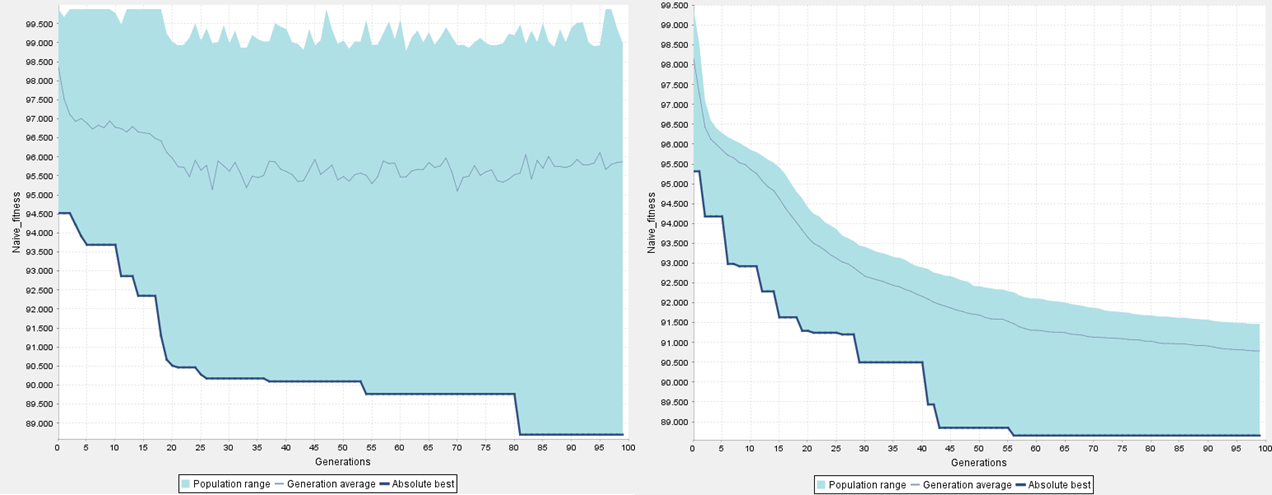
\includegraphics[width=\textwidth]{comparacion-elite}
\caption{A la izquierda gráfica de la evolución de la población con el nuevo método de elitismo. A la derecha gráfica usando el método de elitismo de JECO usado anteriormente. La línea gris muestra la media del fitness de la población.}
\end{figure}

\subsection{Batch Executor}
Debido al empleo de controladores de fantasmas no deterministas, necesitamos la ejecución de varias partidas con el mismo controlador de Pac-Man para obtener resultados estadísticamente correctos del rendimiento del controlador que ha sido evolucionado. Puesto que aumentar el número de partidas a las que que cada individuo se somete al ser evaluado durante la ejecución del algoritmo evolutivo supone un impacto significativo en el tiempo de ejecución del algoritmo, optamos por ejecutar un número conservativo de partidas al evolucionar la población (unas 30).
 
Una vez ejecutado el algoritmo evolutivo, hacemos que el  mejor individuo juegue mil partidas contra el controlador de fantasma deseado.
 
Gracias a este sistema podemos obtener datos precisos, debido a la gran probabilidad de aleatoriedad que está implementada en los controladores de los fantasmas, manteniendo tiempos de entrenamiento razonables. Cabe destacar el hecho de que a partir de 1000 partidas no se produce ninguna mejora en la precisión de los datos obtenidos.
